\chapter{Forschungsdesign}

\section{Definitionen}

\begin{description}
\item[Geschlecht]
Unter Geschlecht verstehen wir, ob jemand als Frau oder Mann, als
Mädchen oder Bub wahrgenommen wird. Wenn wir von Geschlecht reden,
verwenden wir die Begriffe \emph{weiblich}, \emph{männlich},
\emph{Mädchen}, \emph{Bub}, \emph{Frau} oder \emph{Mann}.
\item[Gender]
Unter Gender verstehen wir das vom Geschlecht abhängige Verhalten. Wenn
ein Mann einer Frau den Vortritt lässt dann macht er \emph{Gender}.
\item[Geschlechterstereotype]
Unter Geschlechterstereotypen verstehen wir kulturelle Vorstellungen
über das, was eine typische Frau bzw. ein typischer Mann ist. Wenn wie
von Geschlechtersterotypen reden, verwenden wir die folgenden Begriffe:
\emph{feminin}, \emph{maskulin}. (Tabelle \ref{stereo})
\item[Geschlechterverhältnis]
Unter Geschlechterverhältnis verstehen wir das Verhältnis von weiblichen
zu männlichen Personen. In unserem Fall hauptsächlich das Verhältnis von
Leserinnen zu Lesern. Ist der Anteil der weiblichen Personen höher, die
ein Buch+handelt es sich um ein weibliches Geschlechterverhältnis. Ist
der Anteil der Buben oder Männer größer, dann ist das
Geschlechterverhältnis männlich. Wenn es weder weiblich noch männlich
ist, ist es neutral.
\item[Leserinnen und Leser]
Wenn wir von Leserinnen und Lesern sprechen, meinen wir in dieser Arbeit
nur die untersuchte Grundgesamtheit, das heißt Leserinnen und Leser in
Österreich, die die 3. oder 4. Schulstufe besuchen.
\end{description}

Wenn Leserinnen \emph{oder} Leser \emph{ohne} die jeweils andere Form
verwendet werden, handelt es sich nur um Mädchen oder Buben.

\section{Fragestellungen}

Aus der Forschung geht klar hervor, dass Mädchen und Buben
unterschiedliche Lesepräferenzen haben. Jedoch sind uns keine Studien
bekannt, die das Verhältnis von Leserinnen zu Lesern bei einzelnen
Büchern untersucht haben. Da wir Merkmale von Kinderbüchern mit dem
Geschlecht der Lesenden in Verbindung bringen wollen, ist diese
Information jedoch unabdingbar. Daraus ergibt sich die erste Frage, die
wir in unserer Forschung beantworten wollen.

\begin{frage}\label{fra:andere}
   Wie schaut das Geschlechterverhältnis der Lesenden bei Kinderbüchern aus?
\end{frage}

Dabei geht es uns nicht um ein genaues Abbild der Bücher, die gelesen
werden. Vorangig möchten wir über einige, viel gelesene Bücher das
Geschlechterverhältnis der Lesenden feststellen.

Kinderbücher lassen sich durch viele Kriterien unterscheiden. Uns
interessiert, ob diese Unterschiede mit dem Geschlecht der Lesenden
zusammen hängt. Daraus ergibt sich die nächste Frage die wir hier
beantworten wollen.

\begin{frage}\label{fra:unterschiede}
Welche Unterschiede in Kinderbüchern hängen mit dem Geschlechterverhältnis zusammen?
\end{frage}

Es gibt einige \emph{Kategorien}, in die man die Merkmale einordnen
kann. Einige der Merkmale beziehen sich nur auf den Text des Buchs. Hier
gibt es wiederum Merkmale die sich auf die Handlung, also im Prinzip auf
das Verhalten der Hauptfigur beziehen. Andere beziehen sich auf das
Setting in dem die Geschichte spielt. Dazu gehören \zB Merkmale die oft
unter dem Begriff \emph{Genre} zusammengefasst werden. Wenn es einen
Zusammenhang der Merkmale eine Buchs und dem Geschlechterverhältnis
gibt, stellt sich die Frage, wie dieses Geschlechterverhältnis zustande
kommt. Dabei gibt es unzählige Wege, wie ein Kind dazu kommt, ein
bestimmtes Buch zu lesen. Jedoch welche \emph{Macht} sorgt dafür, dass
Mädchen und Buben unterschiedliche Bücher lesen? Die Beeinflussenden
Faktoren für die Entscheidung ein Buch zu lesen können viele sein. Es
gibt Faktoren die keine direkten Merkmale eine Buchs sind, wie \zB die
Beeinflussung durch andere Menschen, wie Gleichaltrige, Geschwister oder
Eltern die das Buch gelesen haben, Werbung oder Pflichtliteratur in der
Schule. Aber es gibt auch Faktoren die direkte Merkmale eines Buchs
sind. Bei diesen Merkmalen, denken wir an die Situation, wie jemand
alleine vor einem großen Bücherregal in einem Bücherei oder einer
Bibliothek steht und sich ein Buch aussucht. Welche Merkmale
beeinflussen diese Entscheidung? Wir gehen davon aus, dass hier in den
meisten Fällen keine großen Inhaltsanalysen gemacht werden und
hauptsächlich Merkmale die von außen erkennbar sind, für die
Entscheidung wesentlich sind. Aus dieser Vermutung ergibt sich unsere
letzte Frage.

\begin{frage}\label{fra:merkmale}
Kann man ohne über den Inhalt eines Buchs Bescheid zu wissen, auf das Geschlechtererhältnis der Lesenden schließen?
\end{frage}

\section{Hypothesen}

\subsection{Unterschiede im Leseverhalten}

Ausgehend von \thref{fra:andere}, die nach dem Verhältnis von Leserinnen
zu Lesern fragt, interessiert uns, ob wir so etwas wie
\emph{Mädchenbücher} bzw. \emph{Bubenbücher} feststellen können. Daraus
ergibt sich folgende Hypothese.

\begin{hyp}\label{hyp:andere}
    Mädchen lesen andere Bücher als Buben.
\end{hyp}

Die Literatur zeigt, dass Mädchen eher \emph{erlaubt} ist, sich in
männliche Gefilde vor zu wagen als Buben in weibliche. Darauf baut sich
unsere nächste Annahme, die wir überprüfen wollen auf. Wenn das auch bei
Kinderbücher zu trifft, müssten die Anzahl der Leser stärker mit dem
Verhältnis von Leserinnen zu Lesern zusammen hängen als die Anzahl der
Leserinnen.

\begin{subhyp}\label{hyp:anzahl}
    Die Anzahl der Leser hat einen größeren Einfluss auf das Geschlechterverhältnis der Lesenden als die Anzahl der Leserinnen.
\end{subhyp}

\subsection{Unterschiede bei der Hauptfigur}

\thref{hyp:andere} und \thref{hyp:anzahl} haben die Bücher
unterschieden, jedoch haben sich nicht mit der Frage auseinander
gesetzt, ob und wie sich die Geschichten von einander unterscheiden. Die
Geschichten erzählen die Handlungen einer Hauptfigur auf eine spezielle
Art und Weise. Zuerst konzentrieren wir uns auf die Hauptfigur an sich.
Viele Studien gehen davon aus, dass sich Leserinnen eher mit weiblichen
Hauptfiguren identifizieren und Buben eher mit männlichen Hauptfiguren.
Wir wollen überprüfen, ob sich das auch so im Leseverhalten der Kinder
wiederspiegelt. Daraus ergibt sich folgende Hypothese.

\begin{hyp}\label{h2}
    Es gibt einen Zusammenhang zwischen dem Geschlecht der Hauptfigur
    und dem Geschlecht der Lesenden.
\end{hyp}

Ob es einen Zusammenhang gibt oder nicht, heißt nicht automatisch, dass
die Anzahl der Leserinnen und Leser gleich stark damit zusammen hängen.
Deswegen wollen wir in den folgenden Hypothesen den Zusammenhang für
Leser und Leserinnen einzeln prüfen. Unsere Annahmen sind, dass das
Geschlecht der Lesenden und der Hauptfiguren mit einander zusammenhängt.

\begin{subhyp}\label{h2.1}
       Je größer der Anteil an weiblichen Hauptfiguren,
        desto größer ist der Anteil an Leserinnen.
\end{subhyp}

\begin{subhyp}\label{h2.2}
       Je größer der Anteil an männlichen Hauptfiguren,
        desto größer ist der Anteil an Lesern.
\end{subhyp}

Bei einem Teil unserer Bücher ist das Geschlecht der Hauptfigur nicht
eindeutig zuzuorden. Sei es weil es sich um eine Figur handelt die nicht
eindeutig männlich oder weiblich ist oder weil es einen
Multiprotagonisten gibt. Wir gehen davon aus, dass es bei solchen Bücher
\emph{nicht} öfter von Mädchen oder Buben gelesen werden.

\begin{subhyp}\label{h2.3}
    Der Anteil der Hauptfiguren, die sich nicht eindeutig zuzuordnen lassen,   hat keinen Zusammenhang mit dem Geschlechterverhältnis der Lesenden.
\end{subhyp}

Insgesamt gehen wir wieder, aus den selben Gründen wie bei
\thref{hyp:anzahl} davon aus, dass der Einfluss von Lesern stärker als
der von Leserinnen ist.

\begin{subhyp}\label{h2.4}
   Das Geschlecht der Hauptfiguren hängt mit Anzahl der Leser stärker zusammen als mit der Anzahl der Leserinnen.
\end{subhyp}

Bis jetzt haben wir uns am Geschlecht der Hauptfigur orientiert. Jedoch
das Geschlecht der Hauptfigur sagt noch nichts über die Handlung aus.
Die Handlung ist das Verhalten der Hauptfigur. Wir interessieren uns
besonders von das vom Geschlecht der Lesenden abhängige Verhalten der
Hauptfiguren. Ist dieses Verhalten abhängig von den Lesenden stereotyp?
Daraus ergibt sich folgende Hypothese.

\begin{hyp}\label{h3}
   Es gibt einen Zusammenhang zwischen dem Geschlechterverhältnis der Lesenden
    mit  dem Verhältnis zwischen femininen und maskulinen Verhalten der Hauptfiguren.
\end{hyp}

Gibt es einen Zusammenhang, wäre es durchaus denkbar, dass Hauptfiguren
in Büchern die hauptsächlich Mädchen lesen, mit den stereotypen
Geschlechterbildern brechen. Jedoch es könnte natürlich auch umgekehrt
sein, dass sie sich entsprechend der Stereotypen verhalten. Um das zu
überprüfen stellen wir die nächste Hypothese auf.

\begin{subhyp}\label{h3.1}
    Je größer der Anteil an Leserinnen, umso femininer verhalten sich die Hauptfiguren.
\end{subhyp}

Daraus resultiert, dass mit dem Anteil der Leser die Maskulinität der
Hautpfiguren steigt. In den meisten Studien die sich mit dem Gender von
Hauptfiguren beschäftigen, wird das Gender, nicht wie bei uns indirekt,
über das Geschlechterverhältnis bestimmt, sonder direkt über das
Geschlecht der Hauptfigur. Wenn es einen Zusammenhang zwischen dem
Geschlecht der Hauptfigur und dem Geschlecht der Lesenden gibt, könnte
es sein, dass der Zusammenhang zwischen dem Gender und dem
Geschlechterverhältnis verfälscht wird. Die nächste Hypothese dient, um
diesen möglichen Einfluss zu kontrollieren.

\begin{subhyp}\label{h3.2}
    Der Zusammenhang zwischen Geschlechterverhältnis der Lesenden und dem
    mit dem Verhältnis zwischen femininen und maskulinen Verhalten der Hauptfiguren lässt sich nicht durch das Geschlecht der Hauptfiguren erklären.
\end{subhyp}

\subsection{Verschiedene Arten von Geschichten}

Kinderbücher lassen sich in verschiedene Arten von Büchern einteilen.
Man kann dabei Thematisch oder nach speziellen Kriterien vor gehen. Wir
haben uns in einem ersten Schritt auf die Themen konzentriert und in
einem zweiten nach Kriterien gesucht, bei denen wir einen Zusammenhang
mit dem Geschlecht der Lesenden vermuten. Die erste Hypothese fragt nach
der Unterschiedlichkeit der Themen.

\begin{hyp}\label{hyp:themen}
    Mädchen und Buben interessieren sich für unterschiedliche Themen.
\end{hyp}

In einem zweiten Schritt untersuchen wir wesentliche Aspekte der
Geschichten. Als erste Aspekt ist, ob es sich um eine \emph{Abenteurer-}
oder \emph{Alltagsgeschichte} handelt. Wir gehen davon aus, dass Buben
eher Abenteuergeschichten lesen.

\begin{subhyp}\label{h4.1}
   Abenteuergeschichten werden eher von Buben als von Mädchen gelesen.
\end{subhyp}

In vielen Abenteuergeschichten geht es darum bestimmte Fälle zu lösen.
Doch es gibt auch Alltagsgeschichten in denen es um das Lösen bestimmter
Aufgaben geht. Aus diesem Grund überprüfen wir separat, ob es in
Geschichten um das Lösen von \emph{Quests} geht. Wir gehen davon aus,
dass solch Zielgerichtete Geschichten eher von Buben gelesen werden.

\begin{subhyp}\label{h4.2}
    Geschichten in denen \emph{Quests} vorkommen werden eher von Buben als von Mädchen gelesen.
\end{subhyp}

Der nächste Aspekt dem wir uns zu wenden ist der \emph{Innere Monolog}.
Dabei geht es uns um die Elemente einer Geschichte, die persönliche
Konfrontation in den Mittelpunkt stellen. Können wir im im Buch etwas
von den Gedanken, der psychischen Innenwelt der Hauptfigur erfahren? Wir
wollen überprüfen ob Geschichten, in denen diese Elemente wesentlich
sind, vermehrt von Mädchen gelesen werden.

\begin{subhyp}\label{h4.3}
   Geschichten in denen ein \emph{Innerer Monolog} vorkommt, werden eher von Mädchen gelesen als von Buben.
\end{subhyp}

Der letzte Art von Geschichten bezieht sich auf die Veränderung der
Hauptfigur. Es gibt Kindergeschichten in denen die Hauptfigur bleiben
darf wie sie ist. In anderen Geschichten ist \emph{das Erwachsenwerden}
der Figur wesentlich. In diesen Geschichten muss sich die Hauptfigur
verändern um das Ende des Buchs zu erreichen.

\begin{subhyp}\label{h4.4}
   Geschichten in denen \emph{das Erwachsenwerden} Thema ist,
   werden eher von Mädchen als von Buben gelesen.
\end{subhyp}

\subsection{Merkmale die das Geschlechterverhältnis beeinflussen}

In \thref{fra:merkmale} haben wir gefragt, ob man von äußeren Merkmalen
eines Buchs, auf das Geschlechterverhältnis der Lesenden schließen kann.
Daraus leitet sich direkt auch schon die erste Hypothese zu diesem
Bereich ab.

\begin{hyp}\label{h5}
    Man kann das Geschlechterverhältnis durch rein äußere Merkmale eines Buchs erklären.
\end{hyp}

Die zweite Hypothese überprüft ob die Häufigkeit von Mädchen und Buben
auf die selben Merkmale reagiert oder ob es Unterschiede zwischen den
Geschlechtern gibt.

\begin{subhyp}\label{h5.1}
    Die Anzahl der Leserinnen lässt sich besser durch andere Merkmale erklären als die Anzahl der Leser.
\end{subhyp}

\section{Methoden}

\subsection{Fragebogen}

Um \thref{hyp:andere} zu testen, müssen wir zuerst herausfinden, welche
Bücher von welchem Geschlecht gelesen werden. Es gibt zwar Studien, die
sich damit beschäftigen, welche Bücher Mädchen bzw. Buben gerne lesen,
jedoch um einen Unterschied bei der Auswahl der Bücher nachzuweisen,
müssen wir die Daten selbst erheben. Dazu verwenden wir einen Fragebogen
mit dem wir Kinder der 3. und 4. Schulstufe (8--10 Jahre) fragen, welche
Bücher sie bereits gelesen haben. Wir können anhand verschiedener
Studien davon ausgehen , dass Kinder heutzutage immer weniger Lesen.
Weiters ist das Lesegeschwindigkeit und die Schreibgeschwindigkeit bei
vielen Kindern in diesem Alter sehr langsam. Da wir um statistisch
signifikante Aussagen machen zu können pro Buch möglichst viele
\emph{Treffer} benötigen, ist das Design des Fragebogens eine besondere
Herausforderung. Auf Grund dieser Tatsachen entschieden wir uns den
Kindern eine Liste von Büchern vorzulegen, bei denen sie nur noch
Ankreuzen mussten. Die Liste der Bücher erstellten wir anhand von
Bestsellerlisten, der Analyse der Vierleihdaten einer Schulbibliothek
und dem Gespräch mit Volksschullehrerinnen, Bibliothekarinnen und
Buchhändlerinnen. Ergebnis ist eine Liste von 39 Büchern (sieh
Fragebogen auf Seite \pageref{frabo2}) von denen wir ausgehen, das die
Trefferwahrscheinlichkeit akzeptabel ist. Zusätzlich dazu fragen wir die
Lieblingsbücher der Kinder davor in einer offenen Frage ab. Sonst ist
für die Hypothese auf dem Fragebogen nur noch das Geschlecht relevant.

Alle anderen Hypothesen bauen auf die Daten, die wir mit der hier
beschriebenen Methode gewinnen auf. Ausgenommen \thref{hyp:themen}, für
die wir zusätzlich noch Lieblings-Themen, wie \emph{Prinzessinen} oder
\emph{Ritter} abfragen. (Siehe Abbildung \ref{frabo4}) Die Befragungen
werden wärend dem Unterricht in Volksschulen in Graz durchgeführt. Bei
der Auswahl der Volksschulen achteten wir darauf möglichst viele
verschiedenen Milieus abzudecken. Es sollen insgesamt 500 Kinder befragt
werden.

\subsection{Unterschiede im Leseverhalten}

Mit einem $\chi^2$-Vierfeldertest stellen wir für jedes Buch, das
insgesamt mehr als 50 Nennungen hat fest ob ein signifikanter
Unterschied zwischen der Anzahl der Leserinnen und der Anzahl der Lesern
besteht. Danach können wir \thref{hyp:andere} beantworten. Für
\thref{hyp:themen} gehen wir gleich vor und testen ob das Geschlecht das
Interesse für Themen beeinflusst.

Um \thref{hyp:anzahl} zu überprüfen benötigen wir einen Wert der das
Geschlechterverhältnis der Lesenden angibt. Wir bildeten dafür eine
Skala die von $-1$ bis $1$ geht. $-1$ heißt, dass ein Buch nur von
Mädchen gelesen wird. $1$ heißt, dass das Buch nur von Buben gelesen
wird. Mit Hilfe dieser Skala wird ein Faktor, den wir \emph{w/m-Faktor}
oder kurz \emph{w/m} nennen, wird wie folgt gebildet.

\begin{equation}
    w/m=\frac{Buben-Mädchen}{Mädchen+Buben}
\end{equation}

Es gilt zu überprüfen, wie viel die Anzahl der Leserinnen bzw. die
Anzahl der Leser zu diesem Faktor beitragen. Dafür stellen wir ein
multiples lineares Modell auf in dem die und vergleichen die
$\beta$-Werte. Ist der $\beta$-Wert der Buben höher können wir die
\thref{hyp:anzahl} bestätigen.

\subsection{Hauptfigur}

Die nächsten Hypothesen beschäftigen sich mit der \emph{Hauptfigur}. Im
ersten Schritt muss die Hauptfigur festgestellt werden, und dann können
ihr Merkmale zugeordnet werden. Wie bereits im Literaturteil erwähnt
gehen wir davon aus, dass jede Geschichte \emph{eine} Protagonistin oder
\emph{einen} Protagonisten hat. Es kann sich dabei auch um einen
Multiprotagonisten, wie \zB eine Bande handeln. Die Hauptfiguren werden
dann mit Merkmalen versehen. Für \thref{h2} bis \thref{h2.2} brauchen
wir nur das Merkmal Geschlecht. Das kann entweder eindeutig
\emph{weiblich} oder \emph{männlich} sein oder es kann \emph{unbestimmt}
sein. Für \thref{h2} modellieren wir wieder eine lineare Multiple
Regression, wobei das Geschlecht der Hauptfigur in
\emph{Dummy-Variablen} umkodiert werden muss. Für \thref{h2.1} bis
\thref{h2.3} berechnen wir eine Korrelation aus der jeweiligen
Dummy-Variable des Geschlechts der Hauptfigur und dem \emph{w/m-Faktor}
aus. Für \thref{h2.4} benötigen wir zwei Modelle die wir miteinander
Vergleichen. Die Modelle erklären mit Hilfe dem Geschlecht der
Hauptfigur (Dummy-Variablen) die Häufigkeit mit der Mädchen/Buben ein
Buch lesen. Danach vergleichen wir die beiden Modelle mit einer ANOVA.

Für \thref{h3} benötigen wir eine neues Merkmal, dass das Verhalten der
Hauptfigur beschreibt. Und zwar ob das Verhalten \emph{feminin} oder
\emph{maskulin} ist. Um das Verhalten der Hauptfigur zu messen, bilden
wir mit der Hilfe einer Tabelle von eschlechterstereotypen
Gegensatzpaaren ein semantisches Differenzial.
\parencites[174\psq]{feldmann2006}[93\psqq]{Spillner1974} Für jede
Hauptfigur probieren wir jedes Gegensatzpaar zuzuordnen. Dabei bezieht
sich die Zuordnung immer auf das Verhalten/Handeln der Hauptfigur. Um
die Güte der Codierung zu überprüfen wird jede Hauptfigur von zwei
Personen codiert und die Ergebnisse gegenseitig kontrolliert.



      \ctable[
      %  cap    = ,
        caption = {Geschlechterstereotype},
        label   = stereo ,
        % pos   = htp,
      %  width    = \textwidth
      ]{ll}{
        \tnote{Quelle: \inparencite[175]{feldmann2006}}
      }{                  
      \FL {\small weibliche Stereotype} &  {\small männliche Stereotype}
      \ML unterwürfig           & dominant
      \NN abhängig              & unabhängig
      \NN harmonieorientiert/kooperativ & konkurenzorientiert
      \NN passiv                & aktiv/tatkräftig
      \NN sicherheitsbedürftig  & abeteuerlustig/unternehmenslustig
      \NN sanft                 & aggresiv
      \NN furchtsam             & kühn/mutig
      \NN schwach               & stark/kräftig
      \NN träumerisch           & rational/realistisch
      \NN weichherzig/milde     & grausam/hartherzig/streng
      \NN fürsorglich/mütterlich  & egoistisch
      \NN einfühlsam/emotional/gefühlvoll & emotionslos
      \NN unlogisch             & logisch denkend \LL
      }

Aus den Werten wird dann, analog zum \emph{w/m-Faktor} ein, so genannter
\emph{Gender-Faktor} gebildet. haben wir angelehnt an den
\emph{w/m-Faktor} einen Faktor gebildet, der das Verhalten auf einer
Skala von $-1$ (feminin) bis $1$ (maskulin) darstellt. Die
\emph{Gender-Faktor} wird wie folgt berechten. Wobei $m_i$ den einzelnen
Werten ($1=$ feminin, $2=$ maskulin) der 13 Gegensatzpaaren entspricht.

\begin{equation}
    gender=\Bigg(\frac{1}{13}\sum_{i=1}^{13}m_i-1{,}5\Bigg)2
\end{equation}

Danach wird die Korrelation zwischen dem \emph{w/m-Faktor} und dem
\emph{Gender-Faktor} berechnet. Bei \thref{h3.1} wird eine Korrelation
zwischen der Häufigkeit der Leserinnen und dem \emph{Gender-Faktor}
gerechnet. Um gemäß \thref{h3.2} wird der Zusammenhang mit Hilfe der
Dummy-Variablen des Geschlechts der Hauptfigur mit einer
Partialkorrelation kontrolliert.

\subsection{Arten von Geschichten}

Für die \thref{h4.1} bis \thref{h4.4} müssen wir uns genauer mit den
Eigenschaften der Bücher, die hier überprüft werden sollen beschäftigen
und diese operationalisieren. Die erste Eigenschaft ist, ob die
Geschichte ein \emph{Abenteuer} ist.
\blockcquote[Hervorhebung P.\,F.]{wiki_abent}{Als \emph{Abenteuer} \textelp{} wird eine risikoreiche Unternehmung oder auch ein Erlebnis bezeichnet, das sich stark vom \emph{Alltag} unterscheidet -- ein Verlassen des gewohnten Umfeldes und des sozialen Netzwerkes, um etwas (Riskantes) zu unternehmen, was interessant, faszinierend zu sein verspricht und bei dem der Ausgang ungewiss ist.}
Nach der Definition, kann es nur entweder \emph{Abenteuer} oder
\emph{Alltag} geben. Somit gilt es, bei der Geschichte festzustellen, ob
es ein Abenteuer ist oder nicht. Die zweite Eigenschaft nennen wir
\emph{Quest}. Damit meinen wir das gezielte Lösen von Aufgaben, wie sie
\zB in Krimis vorkommen. Die nächste Eigenschaft bezeichnen wir
\emph{Innerer Monolog}, das heißt Textstellen, in denen wir die Gedanken
der Hauptfigur lesen können. Der letzte Eigenschaft von Geschichten
nennen wir \emph{Growing Up}. Damit meinen wir Geschichten in denen die
Hauptfigur (er-)wachsen muss, um ans Ziel zu kommen. Bei all den vier
Punkten geht es um \emph{wesentliche} Elemente der Geschichten.
Natürlich kommt auch in Abenteuer kurz mal der Alltag vor. Hier liegt es
im Ermessen der Coodierenden, ob ein Element wesentlich ist. Um die Güte
dieser Messung zu steigern wird auch hier jedes Element von zwei
Personen unabhängig von einander gemessen. Für die Hypothesen, wird dann
bei jedem Element gleich verfahren und ein, wenn die Fallzahl groß genug
ist, $\chi^2$-Vierfeldertest gerechnet.

\subsection{Erklärung des w/m-Faktors}

Um zu überprüfen welche äußeren Faktoren am meisten zu Erklärung des
Geschlechterverhhältnis der Lesenden und der Anzahl der Leserinnen oder
Leser beitragen stellen wir wieder lineare Multiple Modelle auf, die wir
dann mit Hilfe einer ANOVA mit einander vergleichen.

\chapter{Unterschiedliche Lesepräferenzen von Mädchen und Buben}

In diesem Kapitel wollen wir herausfinden, welche Bücher im Allgemeinen
gerne und häufig gelesen werden, um in einem weiteren Schritt zu
überprüfen ob es Bücher gibt, die von einem Geschlecht tendentiell
bevorzugt werden. Ebenso sollen Vorlieben von Mädchen und Buben
bezüglich der Thematiken in der Kinderliteratur erhoben werden. Anhand
der Ergebnisse soll dann eine Auswahl der Bücher getroffen werden, die,
im Hinblick auf unsere Fragestellungen, interessant sind und weiter
bearbeitet werden sollen.

\section{Erhebung der Lesepräferenzen anhand einer Fragebogenanalyse}

Um herauszufinden, was Buben und Mädchen lesen, liegt eine
Fragebogenanalyse am nächsten. Unsere Stichprobe bildeten
Volksschulkinder der dritten und vierten Klassen in Graz. Die Schulen,
die sich daran beteiligt haben, waren die ``VS Bertha von Suttner'',die
``VS Afritsch'' (davon 2 weitere Klassen am Standort Rosenberggürtel),
die ``VS Engelsdorf'', die ``VS Leopoldinum'', die ``VS Mariatrost'' und
die Prvatschule der``VS Ursulinen''.

Zur Erstellung des Fragebogens muss hinzugefügt werden, dass wir
zusätzlich zu einer offenen Frage (\emph{Was ist dein Lieblingsbuch?})
eine Liste mit Büchern, von denen wir annahmen, dass sie häufig gelesen
werden, zum Ankreuzen verwendeten und noch eine weitere geschlossene
Frage (\emph{Über welche Themen liest du gerne?}) angeboten haben. Zur
Erstellung unserer Bücherliste verwendeten wir hauptsächlich
Bestsellerlisten, zum Teil von Amazon, Ausleihstatistiken von
Bibliotheken und die Expertise einer Mitarbeiterin einer Buchhandlung.
Obwohl wir uns auf Kinder der dritten und vierten Schulstufe
beschränkten, waren auch Bücher in der Auswahl enthalten, die eher die
Funktion eines Vorlese- oder Erstlesebuchs erfüllen. Das hatte den
einfachen Grund auch Schülern und Schülerinnen, die nicht so viel lesen
oder sich auf einem weniger hohen Leseniveau befinden (wir waren auch in
Klassen mit hohen Migrationsanteil und in einer Integrationsklasse),
etwas anzubieten. Außerdem interessierte uns auch, ob und wie sich
Rollenangebote in den Büchern mit steigendem empfohlenem Lesealter
verändern. Der Vorteil einer Liste bestand für uns darin, eine gewisse
Breite an Büchern abzudecken und einer möglichen Schreibfaulheit der
Schüler und Schülerinnen entgegenzukommen, aber auch um Bücher, die vor
einiger Zeit gelesen und eventuell in Vergessenheit geraten waren, zu
repräsentieren. Bei offenen Fragen ist das Problem größer, die Frage
gemeinsam mit dem Nachbarn oder der Nachbarin zu beantworten, was
unserer Annahme nach insgesamt weniger und dafür mehr gleiche Antworten
produziert. Natürlich ist auch eine vorgefertigte Liste nicht frei von
ungewollten Ergebnissen: die Schüler und Schülerinnen könnten möglichst
viel ankreuzen, damit sie vielleicht besser dastehen, genauso gut
zusammenarbeiten oder auch Bücher, die sie nur von Fernsehserien oder
Filmen kennen, angeben. Außerdem kann ein Bias entstehen, wenn etwa eine
Klasse ein bestimmtes Buch auf der Literaturliste hatte und das jeder
Schüler und jede Schülerin sowieso lesen musste. Nach der Durchführung
eines Pretests wurden noch Einzelheiten im Fragebogen verändert. Danach
war es uns möglich, einzuschätzen, ob die Gestaltung des Bogens
überhaupt verständlich und adäquat ist und wie lange Kinder in diesem
Alter brauchen, um einen Bogen auszufüllen. Die Anzahl der Bücher
erschien uns passend, gleich wie die Auswahl der Titel.

\subsection{Auswertung und Ergebnisse}

Wir führten die Fragebogenerhebung gemeinsam mit einer zweiten Gruppe
unseres Forschungsprojekts, die sich mit Fernsehserien beschäftigte,
durch. Auch die Dateneingabe erfolgte in der Großgruppe: Es war wichtig
für jedes Buch und für jede Serie, das/die in der offenen Fragen genannt
wurde, eine eigene Variable zu bilden. Die Aufteilung, Kompatibilität
und Vollständigkeit stellten kein Problem dar. Insgesamt konnten wir mit
502 ausgefüllten Fragebögen (240 von Mädchen, 258 von Buben und vier
ohne Angabe des Geschlechts) aus zwanzig Klassen unsere ersten
Auswertungen beginnen. In die nähere Auswahl gelangten dann nur Bücher,
die mindestens fünfzig Nennungen aufwiesen um die Auswahl zu reduzieren
und die am häufigsten gelesenen hervorzuheben. Mithilfe von
Häufigkeitsanalysen konnten wir unsere vorhandene Liste dann erstmals
von siebenunddreißig auf dreißig Titel einschränken. Weitere
Ausschlusskriterien waren die Altersempfehlung und die Seitenanzahl.
Titel, die einen Bilderbuch- oder Erstlesecharakter aufweisen können mit
denen, die im Normalfall erst ab der zweiten Klasse gelesen werden,
nicht sinnvoll verglichen werden. Ausgeschlossen wurden im Detail
\emph{Der kleine Drache Kokosnuss}, \emph{Der Grüffelo}, \emph{Die
Geggies}, \emph{Der Regenbogenfisch}, \emph{Baumhausgeschichten},
\emph{Das kleine Wutmonster} und \emph{Der kleine Eisbär}.
\emph{Prinzessin Lillifee} ist zwar gerade was die Gestaltung der Bücher
und einer großen Palette von anderen Konsumartikeln betrifft sehr
mädchenhaft (glitzernd und rosa) und ein interessantes Phänomen, aber
wir können nicht annehmen, dass Mädchen in der befragten Altersstufe
diese Bücher noch durchblättern. Bei den \emph{Conni}- Büchern gibt es
verschiedene Autorinnen, die auch für verschiedene Altersspannen
schreiben. Wir haben hier die Bände von Julia Boehme ausgewählt, die
gerade für die dritte und vierte Klasse interessant sind und ließen die
Reihe von Liliane Schneider, die dem Bilderbuchformat entsprechen wie
auch die \emph{Conni \& Co}- Bände, die die Erlebnisse der Conni im
Teenageralter erzählen, unberücksichtigt. \emph{Der kleine Ritter Trenk}
wurde in der Liste gelassen: Obwohl die Altersempfehlung (von 6 bis 8
Jahren) nicht unserern Kriterien entspricht, umfasst das Buch 280 Seiten
und wurde auch mehrmals als Lieblingsbuch angegeben. Bei
\emph{Pinocchio} gibt es verschiedene Ausgaben für ältere sowie für
Kinder im Erstlesealter. Die Geschichte stellt für den Prozess des
Erwachsenwerdens (Growing- Up), auf den später noch näher eingegangen
wird, ein gutes Beispiel dar.

Erst dann sahen wir uns die Verhältnisse, also Nennungen von Buben und
Mädchen separat an. Die Ergebnisse sind in der Tabelle unten
dargestellt, hier wird neben den absoluten Lesehäufigkeiten ein Faktor
errechnet, der ausdrücken soll, ab wann es sich um ein Buben- oder
Mädchenbuch handelt, ob sozusagen Leser ode Leserinnen deutlich
überwiegen oder nicht. Für die Berechnung des „w/m-Faktors``
subtrahierten wir die Anzahl der Nennungen von Mädchen von der Anzahl
der Nennungen bei den Buben und dividierten das Ergebnis durch die
Anzahl der Gesamtnannungen.Die Werte gehen hier theoretisch von $1$
(alle Leser sind Buben = Bubenbuch), bis $-1$ (ausschließlich Leserinnen
= Mädchenbuch).

      \small
      \ctable[
      %  cap    = ,
        caption = {Bücher die über 50 mal genannt wurden},
        label   = top30 ,
        % pos   = htp,
      %  width    = \textwidth
      ]{lD{,}{,}{0}D{,}{,}{0}D{,}{,}{0}D{,}{,}{2}}{
        \tnote{--1: 100\% Leserinnen; 0: gleich viele Leserinnen wie Leser; 1: 100\% Leser}
      % \tnote[.]{< 0,1}
      % \tnote[*]{< 0,05}
      % \tnote[**]{< 0,01}
      % \tnote[***]{< 0,001}
      }{                  
      \FL \footnotesize Bücher &  \multicolumn{1}{c}{\footnotesize Mädchen} & \multicolumn{1}{c}{\footnotesize Buben} & \multicolumn{1}{c}{\footnotesize Gesamt} & \multicolumn{1}{c}{ \footnotesize w/m-Faktor\tmark}
      \ML Die wilden Fußballkerle & 43 & 110 & 153 & 0,44\tmark[**]% 18  $ 0,00 **
      \NN Tiger-Team & 49 & 69 & 118 & 0,17
      \NN Knickerbocker-Bande & 48 & 67 & 115 & 0,17
      \NN Gregs Tagebuch & 86 & 117 & 203 & 0,15\tmark[*]% 28  $ 0,03 *
      \NN Harry Potter & 95 & 125 & 220 & 0,14\tmark[$\circ$]% 29  $ 0,05 .
      \NN Die drei ??? & 93 & 122 & 215 & 0,14\tmark[$\circ$]% 27  $ 0,05 .
      \NN Das magische Baumhaus & 84 & 105 & 189 & 0,11
      \NN Der kleine Ritter Trenk & 42 & 52 & 94 & 0,11
      \NN Tom Turbo & 92 & 113 & 205 & 0,10
      \NN Der kleine Drache Kokosnuss & 46 & 52 & 98 & 0,06
      \NN Der Räuber Hotzenplotz & 92 & 101 & 193 & 0,05
      \NN Sams & 63 & 67 & 130 & 0,03
      \NN Fünf Freunde & 114 & 118 & 232 & 0,02
      \NN Die Olchis & 47 & 48 & 95 & 0,01
      \NN Der Grüffelo & 58 & 54 & 112 & -0,04
      \NN Die Geggis & 36 & 31 & 67 & -0,08
      \NN Peter Pan & 90 & 73 & 163 & -0,10\tmark[*]% 15  $ 0,03 *
      \NN Der Regenbogenfisch & 122 & 95 & 217 & -0,12\tmark[**]% 1   $ 0,00 **
      \NN Baumhausgeschichten & 29 & 22 & 51 & -0,14
      \NN Geschichten von Franz & 83 & 60 & 143 & -0,16\tmark[*]% 16  $ 0,01 *
      \NN Pinocchio & 96 & 68 & 164 & -0,17\tmark[**]% 14  $ 0,00 **
      \NN Das kleine Wutmonster & 34 & 23 & 57 & -0,19% 7   $ 0,07 .
      \NN Der kleine Eisbär & 91 & 56 & 147 & -0,24\tmark[**]% 10  $ 0,00 **
      \NN Pipi Langstrumpf & 141 & 75 & 216 & -0,31\tmark[**]% 32  $ 0,00 **
      \NN Die kleine Hexe & 109 & 52 & 161 & -0,35\tmark[**]% 11  $ 0,00 **
      \NN Hexe Lilli & 162 & 53 & 215 & -0,51\tmark[**]% 35  $ 0,00 **
      \NN Die wilden Hühner & 77 & 25 & 10 & -0,51\tmark[**]% 24  $ 0,00 **
      \NN Mini & 59 & 16 & 75 & -0,57\tmark[**]% 36  $ 0,00 **
      \NN Conni & 94 & 22 & 116 & -0,62\tmark[**]% 37  $ 0,00 **
      \NN Prinzessin Lillifee & 109 & 14 & 123& -0,77\tmark[**]% 17  $ 0,00 **  
      \LL \multicolumn{5}{l}{\footnotesize $^\circ p<0{,}1, ^*p<0{,}05, ^{**}p<0{,}01$ $\chi^2$-Test (Mädchen/Buben) $N=498$}
      }
      

\normalsize

% 1   $ 0,00 **
% 3   $ 0,85
% 4   $ 0,33
% 5   $ 0,39
% 7   $ 0,07 .
% 10  $ 0,00 **
% 11  $ 0,00 **
% 13  $ 0,45
% 14  $ 0,00 **
% 15  $ 0,03 *
% 16  $ 0,01 *
% 17  $ 0,00 **
% 18  $ 0,00 **
% 19  $ 0,22
% 20  $ 0,97
% 21  $ 0,19
% 22  $ 0,10
% 23  $ 0,11
% 24  $ 0,00 **
% 25  $ 0,78
% 26  $ 0,69
% 27  $ 0,05 .
% 28  $ 0,03 *
% 29  $ 0,05 .
% 32  $ 0,00 **
% 33  $ 0,78
% 34  $ 0,19
% 35  $ 0,00 **
% 36  $ 0,00 **
% 37  $ 0,00 **

% N=498

Obwohl Titel, die in der offenen Frage angegeben wurden, nicht in die
weitere Auswahl kamen, erwies sich die offene
\emph{Lieblingsbücher}-Frage dennoch als sinnvoll, um die Bücherauswahl
zu kontrollieren. Die höchste Anzahl an Nennungen bei der offenen Frage
bekamen die \emph{Lustigen Taschenbücher} mit vierzehn, was leider nicht
als repräsentativ angesehen werden kann. Die anderen
\emph{Lieblingsbücher} zählten höchstens fünf Nennungen insgesamt.

Schon auf den ersten Blick auf die Tabelle ist leicht zu erkennen, dass
Mädchenbücher eindeutiger als Mädchenbücher gelten können, als das bei
Bubenbüchern der Fall ist: Buben präferieren eindeutig \emph{Die wilden
Fußballkerle} mit einem Wert von über 0,4. Dann kommt erst mit einem
Wert von 0,17 das \emph{Tiger- Team}, \emph{Die Knickerbockerbande} und
\emph{Gregs Tagebuch} (0,15). Bei den Mädchen können wir die Zahlen viel
eindeutiger interpretieren, da ihre Werte näher am Extremwert
angesiedelt sind. \emph{Conni} führt die Liste mit einem Wert von -0,62
an, es folgen , \emph{Geschichten von Mini} (-0,57), \emph{Die wilden
Hühner} (0,51) und \emph{Hexe Lilli} (0,51). Dieser w/m- Faktor ist aber
immer noch höher, als der von dem eindeutigsten Bubenbuch.

Kann angenommen werden, dass die beliebtesten Bücher klare Mädchen- oder
Bubenbücher sind oder handelt es sich bei ihnen um ausgewogene
Verhältnisse? Am beliebtesten beziehungsweise insgesamt am häufigsten
gelesen wurden die \emph{5 Freunde} mit 232 Nennungen. Dabei handelt es
sich um Bände, die keine klare Präferenz von Seiten der Buben oder
Mädchen aufweisen. Dann folgt \emph{Harry Potter}, wo Unterschiede nur
tendenziell zugunsten der Buben interpretiert werden könnten, wir es
aufgrund der hohen Leserinnenanzahl aber nicht als Bubenbuch definieren
wollen. \emph{Pippi Langstrumpf} und \emph{Die Hexe Lilli}können
aufgrund der hohen Gesamtanzahl und der klaren weiblichen Bevorzugung
als eindeutige Mädchenbücher definiert werden. \emph{Gregs Tagebuch}
steht an siebenter Stelle mit 203 Nennungen und wird von Buben bevorzugt
gelesen.

      
      \ctable[
      %  cap    = ,
        caption = {Lineares Modell, dass den unterschiedlichen Einfluss von Mädchen und Buben auf das Geschlechterverhältnis zeigt},
        label   = wmbm ,
        % pos   = htp,
       width    = 7cm
      ]{lD{,}{,}{2}}{
        % \tnote[.]{< 0,1}
        % \tnote[*]{< 0,05}
        % \tnote[**]{< 0,01}
        % \tnote[***]{< 0,001}
      }{                  
      \FL 
      \small   &  
      \multicolumn{1}{c}{\small Modell}
      \ML Anzahl der Leserinnen     & -0,61\tmark[***] 
      \NN Anzahl der Leser          &  0,83\tmark[***]   
      \ML Korrigiertes $R^2$        &  0,89\tmark[***]      
      \LL \multicolumn{2}{l}{\footnotesize  $^*p<0{,}05, ^{**}p<0{,}01, ^{***}p<0{,}001$}
      }
      

Weitere interessante Ergebnisse lieferte die Auswertung der Frage zu
Themen, die Mädchen und Buben interessieren könnten. Dabei sind wir nach
dem gleichen Schema wie bei den einzelnen Titeln vorgegangen, weshalb
die folgende Tabelle gleich gelesen werden kann wie die obere.
Interessant ist, dass kein einziger Bub angegeben hat, gerne etwas über
Prinzessinnen zu lesen. Literatur, die sich um dieses Thema dreht, ist
eindeutig weiblich konnotiert, wahrscheinlich würde sich ein Junge
schämen, wenn man irgendetwas \emph{prinzessinnenhaftes} bei ihm
entdecken würde. Das erweckt den Eindruck, dass Buben sehr
mädchentypische Dinge stark ablehnen. Die Vermutung, dass Mädchen sich
eher für Freundschaft und Liebe interessieren (und sich das auch angeben
trauen), hat sich mit diesem Ergebnis bestätigt: Dabei kann eine
stärkere ``Beziehungsorientierung'' des weiblichen Geschlechts schon im
frühen Alter bestätigt werden. Auch Tiere, die eher im niedlicheren
Bereich eingeschätzt werden, finden bei den Mädchen eine klare
Bevorzugung. Buben favorisieren hingegen den technischen Bereich, auch
Drachen und Ritter sind für sie interessant. Wir vermuteten ursprünglich
hingegen eine stärkere Ablehnung von Mädchen im Bereich Fußball und
Sport.

     \small
      \ctable[
      %  cap    = ,
        caption = {Welche Themen liest du gerne?},
        label   = themen ,
        star,
        % pos   = htp,
      %  width    = \textwidth
      ]{lD{,}{,}{0}D{,}{,}{0}D{,}{,}{0}D{,}{,}{3}}{
        \tnote{--1: 100\% Leserinnen; 0: gleich viele Leserinnen wie Leser; 1: 100\% Leser}
      }{                  
      \FL \footnotesize Themen &  \multicolumn{1}{c}{\footnotesize Mädchen} & \multicolumn{1}{c}{\footnotesize Buben} & \multicolumn{1}{c}{\footnotesize Gesamt} & \multicolumn{1}{c}{ \footnotesize w/m-Faktor\tmark}
      \ML Autos/Technik & 16 & 130 & 146 & 0,78\tmark[**]
      \NN Drachen/Ritter & 44 & 107 & 151 & 0,68\tmark[**]
      \NN Dinosaurier & 32 & 87 & 119 & 0,46\tmark[**]
      \NN Fußball/Sport & 67 & 173 & 240 & 0,44\tmark[**]
      \NN Abenteuer/Indianer/Piraten & 77 & 116 & 193 & 0,20\tmark[**]
      \NN Geister/Monster & 97 & 122 & 219 & 0,11%
      \NN Meerestiere & 92 & 77 & 169 & -0,09\tmark[*]
      \NN Hexen/Zauberer & 114 & 52 & 166 & -0,37\tmark[**]
      \NN Pferde, Hunde, Katzen & 145 & 52 & 166 & -0,37\tmark[**]
      \NN Freunde/Liebe & 108 & 23 & 132 & -0,64\tmark[**]
      \NN Prinzessinen & 53 & 0 & 53& -1,00\tmark[**]  
      \LL \multicolumn{5}{l}{\footnotesize $^*p<0{,}05, ^{**}p<0{,}01$ $\chi^2$-Test (Mädchen/Buben) $N=498$}
      }
      \normalsize

Problematisch beim Fragebogen im Nachhinein war, dass die Bücherauswahl
doch einen weiten Range abdeckt und Titel deshalb auch teilweise schwer
miteinander zu vergleichen sind. Bei Harry Potter und dem
Regenbogenfisch würde der Versuch ad absurdum führen. Außerdem stehen
den Kindern neben Klassikern, die seit Jahrzehnten gelesen werden
(\emph{Fünf Freunde}, \emph{Pippi Langstrumpf}) auch eine große Auswahl
an neuen Büchern zur Verfügung ( \emph{Gregs Tagebuch}, \emph{Die wilden
Fußballkerle}). Nach einer gründlicheren Recherche und Literaturanalyse,
hätte man aus dem Fragebogen etwas mehr herausholen können. Außerdem
wurden Sachbücher aufgrund eines fehlenden Hauptcharkters nicht
berücksichtigt, die in diesem Alter gerade von Buben gerne gelesen
werden und die auch Themenvorlieben gut repräsentieren könnten. Auch die
Auswahl kann, trotz Änderungen und Verbesserungen unsererseits,
Verzerrungen aufweisen, da bei diesem Umfang der Liste von vornherein
Vieles ausgeschlossen werden musste.

\subsection{Interpretation der Ergebnisse}

Bei den vorherigen Recherchen stießen wir immer wieder auf Ergebnisse
von PISA oder ähnlichen Studen, die darauf hinwiesen, dass Burschen
deutlich weniger lesen würden als Mädchen und auch eher mit
Leseschwächen zu kämpfen hätten, was aber allein anhand unseres
Fragebogens nicht nachgewiesen werden kann. Die leicht höhere Anzahl an
Gesamtnennungen bei den Mädchen kann das allein nicht bestätigen.
Unserer Vermutung nach könnte sich die geringere Anzahl an
Gesamtnennungen eventuell mit einem etwas geringere Leseinteresse der
Buben, wie auch einem fehlenden Angebot an Comics oder Sachbüchern (
z.B. \emph{Was ist was?}) in der Liste erklären lassen. Warum aber gibt
es mehr eindeutige Mädchen- als Bubenbücher? Hier liegt die Erklärung
nahe, die sich auch mit Aussagen in der Literatur deckt, dass Mädchen
einen größeren Spielraum haben, wenn es um Interessengebiete oder
Handlungsmöglichkeiten geht. Mädchen sollen sogar weibliche und
männliche Elemente verbinden: starke, wie auch technikversierte Frauen
sind gern gesehen. Diese Entwicklung ist äußerst positiv zu bewerten,
wobei kritisiert werden kann, dass bei Buben diese Flexibilität (noch)
nicht den gleichen Stellenwert erreicht hat. Sie bewegen sich viel
seltener in ``weiblichen Domänen'', als dies Mädchen und Frauen
inzwischen umgekehrt tun.

Die beliebtesten stellen nicht gleichzeitig die eindeutigsten Bücher
dar. Allerdings sind einige unter den viel gelesenen dabei, die in eine
klare Richtung weisen und es deshalb wert sind, auf ihre Besonderheiten
hin, untersucht zu werden.

Für weitere Analysen musste entschieden werden, welche Bände einer Reihe
oder Serie ausgewählt werden. Hier spielte die Aktualität und
Beliebtheit (laut Amazon) eine Rolle. Im Zweifelsfall wurden mehrere
Bücher verglichen. Dabei zeigte sich, dass bei der Darstellung der
Charaktere etwa bei dem \emph{Tiger- Team}, \emph{Der
Knickerbockerbande}, den \emph{5 Freunden}, Geschichten von \emph{Franz}
und \emph{Mini} und auch bei \emph{Conni} keine Unterschiede
festgestellt werden können. Die Liste der verwendeten Bände und Ausgaben
befindet sich im Anhang.

\chapter{Handeln Hauptfiguren in Mädchenbüchern anders als in
Bubenbüchern?}

\section{Inhaltliche Unterschiede}

Da wir in den vorangegangenen Kapiteln zeigen konnten, dass Mädchen und
Buben unterschiedliche Bücher lesen, was zwar klarer bei den Jungen als
bei den Mädchen festgstellt werden konnte, stellt sich dennoch die
Frage, ob es denn auch Unterschiede in den, von den Gruppen
favorisierten, Werken gibt. Dieses Kapitel hat sich zur Aufgabe gemacht,
sich auf die Suche nach inhaltlichen Merkmalen zu machen, die die beiden
Büchergruppen unterscheiden. Untermauert mit inhaltlichen
Interpretationen und Auszügen aus Beispielbüchern soll so ein
Verständnis über diese spezifisch verwendeten Merkmale erzeugt werden um
schließlich Annahmen über mögliche Folgen von derartigen Unterschieden
in den Lesepräferenzen von jungen Menschen zu formulieren. Der Inhalt
der Kinderbücher wurde hierbei auf zwei Ebenen untersucht:

\begin{itemize}
\item
  Unterschiede in der Darstellung des sozialen Geschlechts (Gender) der
  Hauptprotagonisten
\item
  Unterschiede im Aufbau und Verwendung stilistischer Mittel
\end{itemize}

\section{Darstellung Gender}

Auch wenn die Frage nach der Intensität des Einflusses von Kinderbüchern
auf die Sozialisierung und die Ausprägung von Geschlechterrollen bei
Kindern nicht restlos beantwortet werden kann, muss hier dennoch von
einem Einfluss ausgegangen werden. Dieser Einfluss geht vor allem von
den Hauptprotagonisten und deren Verhalten, Handeln und Denken aus. Sie
stellen jene Identifizierungsinstanz dar mit denen im Verlauf der
Geschichte des jeweiligen Buches am meisten mitgelitten, gefeiert und
gebangt wird. Daher ist es von hoher Bedeutung wie diese Charaktere
dargestellt werden. Jene Form der Darstellung, die uns hier im
Besonderen interessiert, ist die des sozialen Geschlechtes, welche mit
Hilfe einer Liste von 13 Eigenschaftspaaren (siehe Tabelle \ref{stereo})
erhoben wurde. Jedes dieser Eigenschaftspaare weist einen stereotyp
maskulinen und femininen Pol auf. Jeder Hauptcharakter der 30 Bücher
unserer Erhebung wurde auf diese 13 Eigenschaftspaare untersucht und ein
Gender-Faktor erstellt, der uns zeigen kann, wie maskulin oder feminin
die Protagonisten dargestellt werden.

      
      \ctable[
      %  cap    = ,
        caption = {w/m-Faktor -- Gender-Faktor},
        label   = top30gender ,
        pos   = htp,
        star,
      %  width    = \textwidth
      ]{lD{,}{,}{2}D{,}{,}{2}}{
        \tnote{--1: 100\% Leserinnen; 0: gleich viele Leserinnen wie Leser; 1: 100\% Leser}
      }{                  
      \FL \small Bücher &  \multicolumn{1}{c}{\small w/m-Faktor} & \multicolumn{1}{c}{ \small Gender-Faktor}
      \ML Die wilden Fußballkerle   & 0,44      & 0,54
      \NN Tiger-Team                & 0,17      &0,15
      \NN Die Knickerbocker-Bande        & 0,16      & 0,31
      \NN Gregs Tagebuch            & 0,15      &0,23
      \NN Harry Potter              & 0,13      &0,23
      \NN Die drei ???              & 0,14      &0,54
      \NN Das magische Baumhaus     & 0,11      &0,50
      \NN Der kleine Ritter Trenk   & 0,11      &0,23
      \NN Tom Turbo                 & 0,10      &0,69
      \NN Der kleine Drache Kokosnuss  & 0,06   &0,08
      \NN Der Räuber Hotzenplotz    & 0,05      &-0,08
      \NN Sams                      & 0,03      &-0,23
      \NN Fünf Freunde              & 0,02      &0,15
      \NN Die Olchis                & 0,01      &-0,15
      % \NN Der Grüffelo              & -0,04     &0,69
      % \NN Die Geggis                & -0,08     &-0,08
      \NN Peter Pan                 & -0,10     &-0,38
      % \NN Der Regenbogenfisch       & -0,12     &0,45
      % \NN Baumhausgeschichten       & -0,14     &-0,15
      \NN Geschichten von Franz     & -0,16     & -0,69
      \NN Pinocchio                 & -0,17     & -0,38
      % \NN Das kleine Wutmonster     & -0,19     & -0,23
      % \NN Der kleine Eisbär         & -0,24     & 0,17
      \NN Pipi Langstrumpf          & -0,31     & 0,08
      \NN Die kleine Hexe           & -0,35     & 0,54
      \NN Hexe Lilli                & -0,51     & 0,08
      \NN Die wilden Hühner         & -0,51     & 0,31
      \NN Mini                      & -0,57     & - 0,31
      \NN Conni                     & -0,62     & -0,62
      % \NN Prinzessin Lillifee       &-0,77      & -0,33  
      \LL
      }
      

Das Lesegeschlecht (w/m-Faktor) korreliert mit dem Gender-Faktor
hochsignifikant mit einem Wert von $r = 0{,}471$. Somit kann die bereits
in der Tabelle erkennbare Tendenz, dass Mädchen vor allem mit femininen
Charakteren sowie Buben vor allem mit maskulinen Charakteren
konfrontiert werden, auch statistisch festgehalten werden. Besonders
interessant ist jedoch dieses Ergebnis erst, wenn wir uns die
Geschlechter im Einzelnen ansehen. In der Abbildung \ref{wm-gender}
sehen wir um wie viel klarer diese Konfrontation bei den Jungen ausfällt
als bei den Mädchen. Dies ist wie folgt zu interpretieren: Beide
Geschlechter lesen vermehrt von sozialen Geschlechtern, die ihrem
eigenen Geschlecht entsprechen. Während jedoch die Buben hier besonders
stark mit maskulinen Protagonisten konfrontiert werden, lesen Mädchen
von Charakteren beider Genderausprägungen. Dies ist wahrscheinlich
einerseits in dem Tabu für Jungen in Mädchendomänen einzudringen
verbunden, anderseits auch mit einem emanzipatorischen Anspruch vieler
Autorinnen verknüpft die ihre Charaktere bewusst untypisch darstellen,
um bestehende Geschlechterverhältnisse aufzubrechen.

\begin{figure}
\center
  \caption[w/m-Faktor--Gender-Faktor]{w/m-Faktor zu Gender-Faktor}
  \label{wm-gender}
% Created by tikzDevice version 0.6.2-92-0ad2792 on 2013-02-07 01:52:29
% !TEX encoding = UTF-8 Unicode
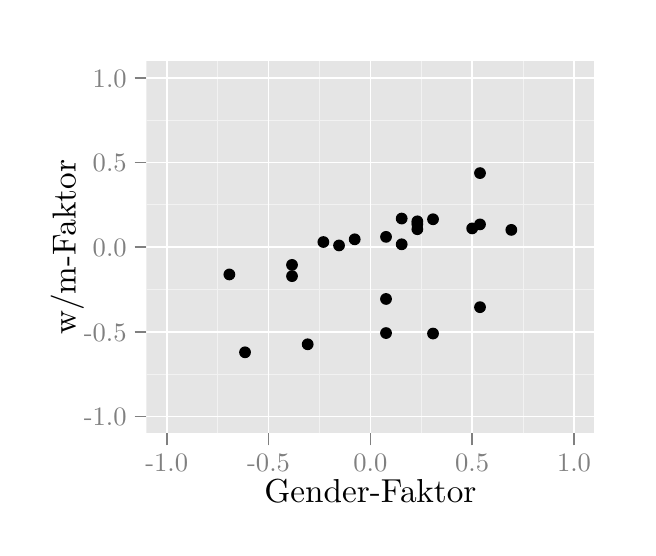
\begin{tikzpicture}[x=1pt,y=1pt]
\definecolor[named]{fillColor}{rgb}{1.00,1.00,1.00}
\path[use as bounding box,fill=fillColor,fill opacity=0.00] (0,0) rectangle (216.81,180.67);
\begin{scope}
\path[clip] (  0.00,  0.00) rectangle (216.81,180.67);
\definecolor[named]{drawColor}{rgb}{1.00,1.00,1.00}
\definecolor[named]{fillColor}{rgb}{1.00,1.00,1.00}

\path[draw=drawColor,line width= 0.6pt,line join=round,line cap=round,fill=fillColor] (  0.00,  0.00) rectangle (216.81,180.68);
\end{scope}
\begin{scope}
\path[clip] ( 42.89, 34.03) rectangle (204.77,168.63);
\definecolor[named]{fillColor}{rgb}{0.90,0.90,0.90}

\path[fill=fillColor] ( 42.89, 34.03) rectangle (204.77,168.63);
\definecolor[named]{drawColor}{rgb}{0.95,0.95,0.95}

\path[draw=drawColor,line width= 0.3pt,line join=round] ( 42.89, 55.45) --
	(204.77, 55.45);

\path[draw=drawColor,line width= 0.3pt,line join=round] ( 42.89, 86.04) --
	(204.77, 86.04);

\path[draw=drawColor,line width= 0.3pt,line join=round] ( 42.89,116.63) --
	(204.77,116.63);

\path[draw=drawColor,line width= 0.3pt,line join=round] ( 42.89,147.22) --
	(204.77,147.22);

\path[draw=drawColor,line width= 0.3pt,line join=round] ( 68.64, 34.03) --
	( 68.64,168.63);

\path[draw=drawColor,line width= 0.3pt,line join=round] (105.43, 34.03) --
	(105.43,168.63);

\path[draw=drawColor,line width= 0.3pt,line join=round] (142.22, 34.03) --
	(142.22,168.63);

\path[draw=drawColor,line width= 0.3pt,line join=round] (179.01, 34.03) --
	(179.01,168.63);
\definecolor[named]{drawColor}{rgb}{1.00,1.00,1.00}

\path[draw=drawColor,line width= 0.6pt,line join=round] ( 42.89, 40.15) --
	(204.77, 40.15);

\path[draw=drawColor,line width= 0.6pt,line join=round] ( 42.89, 70.74) --
	(204.77, 70.74);

\path[draw=drawColor,line width= 0.6pt,line join=round] ( 42.89,101.33) --
	(204.77,101.33);

\path[draw=drawColor,line width= 0.6pt,line join=round] ( 42.89,131.92) --
	(204.77,131.92);

\path[draw=drawColor,line width= 0.6pt,line join=round] ( 42.89,162.51) --
	(204.77,162.51);

\path[draw=drawColor,line width= 0.6pt,line join=round] ( 50.24, 34.03) --
	( 50.24,168.63);

\path[draw=drawColor,line width= 0.6pt,line join=round] ( 87.03, 34.03) --
	( 87.03,168.63);

\path[draw=drawColor,line width= 0.6pt,line join=round] (123.83, 34.03) --
	(123.83,168.63);

\path[draw=drawColor,line width= 0.6pt,line join=round] (160.62, 34.03) --
	(160.62,168.63);

\path[draw=drawColor,line width= 0.6pt,line join=round] (197.41, 34.03) --
	(197.41,168.63);
\definecolor[named]{fillColor}{rgb}{0.00,0.00,0.00}

\path[fill=fillColor] (112.51,101.98) circle (  2.13);

\path[fill=fillColor] (118.17,104.19) circle (  2.13);

\path[fill=fillColor] (129.49,105.08) circle (  2.13);

\path[fill=fillColor] (129.49, 70.32) circle (  2.13);

\path[fill=fillColor] (140.81,107.84) circle (  2.13);

\path[fill=fillColor] (163.45, 79.67) circle (  2.13);

\path[fill=fillColor] ( 78.54, 63.36) circle (  2.13);

\path[fill=fillColor] ( 95.52, 90.89) circle (  2.13);

\path[fill=fillColor] ( 95.52, 94.95) circle (  2.13);

\path[fill=fillColor] (174.77,107.60) circle (  2.13);

\path[fill=fillColor] ( 72.88, 91.49) circle (  2.13);

\path[fill=fillColor] (101.18, 66.26) circle (  2.13);

\path[fill=fillColor] (106.85,103.21) circle (  2.13);

\path[fill=fillColor] (129.49, 82.64) circle (  2.13);

\path[fill=fillColor] (135.15,102.39) circle (  2.13);

\path[fill=fillColor] (135.15,111.70) circle (  2.13);

\path[fill=fillColor] (163.45,128.12) circle (  2.13);

\path[fill=fillColor] (146.47,111.44) circle (  2.13);

\path[fill=fillColor] (140.81,109.67) circle (  2.13);

\path[fill=fillColor] (140.81,110.68) circle (  2.13);

\path[fill=fillColor] (146.47, 70.14) circle (  2.13);

\path[fill=fillColor] (160.62,108.13) circle (  2.13);

\path[fill=fillColor] (163.45,109.58) circle (  2.13);
\end{scope}
\begin{scope}
\path[clip] (  0.00,  0.00) rectangle (216.81,180.67);
\definecolor[named]{drawColor}{rgb}{0.50,0.50,0.50}

\node[text=drawColor,anchor=base east,inner sep=0pt, outer sep=0pt, scale=  0.96] at ( 35.77, 36.85) {-1.0};

\node[text=drawColor,anchor=base east,inner sep=0pt, outer sep=0pt, scale=  0.96] at ( 35.77, 67.44) {-0.5};

\node[text=drawColor,anchor=base east,inner sep=0pt, outer sep=0pt, scale=  0.96] at ( 35.77, 98.03) {0.0};

\node[text=drawColor,anchor=base east,inner sep=0pt, outer sep=0pt, scale=  0.96] at ( 35.77,128.62) {0.5};

\node[text=drawColor,anchor=base east,inner sep=0pt, outer sep=0pt, scale=  0.96] at ( 35.77,159.21) {1.0};
\end{scope}
\begin{scope}
\path[clip] (  0.00,  0.00) rectangle (216.81,180.67);
\definecolor[named]{drawColor}{rgb}{0.50,0.50,0.50}

\path[draw=drawColor,line width= 0.6pt,line join=round] ( 38.62, 40.15) --
	( 42.89, 40.15);

\path[draw=drawColor,line width= 0.6pt,line join=round] ( 38.62, 70.74) --
	( 42.89, 70.74);

\path[draw=drawColor,line width= 0.6pt,line join=round] ( 38.62,101.33) --
	( 42.89,101.33);

\path[draw=drawColor,line width= 0.6pt,line join=round] ( 38.62,131.92) --
	( 42.89,131.92);

\path[draw=drawColor,line width= 0.6pt,line join=round] ( 38.62,162.51) --
	( 42.89,162.51);
\end{scope}
\begin{scope}
\path[clip] (  0.00,  0.00) rectangle (216.81,180.67);
\definecolor[named]{drawColor}{rgb}{0.50,0.50,0.50}

\path[draw=drawColor,line width= 0.6pt,line join=round] ( 50.24, 29.77) --
	( 50.24, 34.03);

\path[draw=drawColor,line width= 0.6pt,line join=round] ( 87.03, 29.77) --
	( 87.03, 34.03);

\path[draw=drawColor,line width= 0.6pt,line join=round] (123.83, 29.77) --
	(123.83, 34.03);

\path[draw=drawColor,line width= 0.6pt,line join=round] (160.62, 29.77) --
	(160.62, 34.03);

\path[draw=drawColor,line width= 0.6pt,line join=round] (197.41, 29.77) --
	(197.41, 34.03);
\end{scope}
\begin{scope}
\path[clip] (  0.00,  0.00) rectangle (216.81,180.67);
\definecolor[named]{drawColor}{rgb}{0.50,0.50,0.50}

\node[text=drawColor,anchor=base,inner sep=0pt, outer sep=0pt, scale=  0.96] at ( 50.24, 20.31) {-1.0};

\node[text=drawColor,anchor=base,inner sep=0pt, outer sep=0pt, scale=  0.96] at ( 87.03, 20.31) {-0.5};

\node[text=drawColor,anchor=base,inner sep=0pt, outer sep=0pt, scale=  0.96] at (123.83, 20.31) {0.0};

\node[text=drawColor,anchor=base,inner sep=0pt, outer sep=0pt, scale=  0.96] at (160.62, 20.31) {0.5};

\node[text=drawColor,anchor=base,inner sep=0pt, outer sep=0pt, scale=  0.96] at (197.41, 20.31) {1.0};
\end{scope}
\begin{scope}
\path[clip] (  0.00,  0.00) rectangle (216.81,180.67);
\definecolor[named]{drawColor}{rgb}{0.00,0.00,0.00}

\node[text=drawColor,anchor=base,inner sep=0pt, outer sep=0pt, scale=  1.20] at (123.83,  9.03) {Gender-Faktor};
\end{scope}
\begin{scope}
\path[clip] (  0.00,  0.00) rectangle (216.81,180.67);
\definecolor[named]{drawColor}{rgb}{0.00,0.00,0.00}

\node[text=drawColor,rotate= 90.00,anchor=base,inner sep=0pt, outer sep=0pt, scale=  1.20] at ( 17.30,101.33) {w/m-Faktor};
\end{scope}
\end{tikzpicture}


\end{figure}

\begin{figure}
\center
  \caption[Mädchen--Gender-Faktor]{Mädchen zu Gender-Faktor}
  \label{w-gender}
% Created by tikzDevice version 0.6.2-92-0ad2792 on 2013-02-07 02:00:58
% !TEX encoding = UTF-8 Unicode
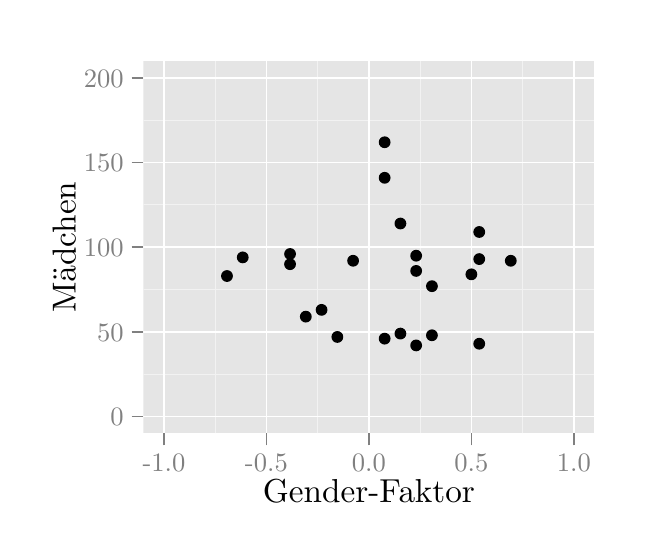
\begin{tikzpicture}[x=1pt,y=1pt]
\definecolor[named]{fillColor}{rgb}{1.00,1.00,1.00}
\path[use as bounding box,fill=fillColor,fill opacity=0.00] (0,0) rectangle (216.81,180.67);
\begin{scope}
\path[clip] (  0.00,  0.00) rectangle (216.81,180.67);
\definecolor[named]{drawColor}{rgb}{1.00,1.00,1.00}
\definecolor[named]{fillColor}{rgb}{1.00,1.00,1.00}

\path[draw=drawColor,line width= 0.6pt,line join=round,line cap=round,fill=fillColor] (  0.00,  0.00) rectangle (216.81,180.68);
\end{scope}
\begin{scope}
\path[clip] ( 41.82, 34.03) rectangle (204.77,168.63);
\definecolor[named]{fillColor}{rgb}{0.90,0.90,0.90}

\path[fill=fillColor] ( 41.82, 34.03) rectangle (204.77,168.63);
\definecolor[named]{drawColor}{rgb}{0.95,0.95,0.95}

\path[draw=drawColor,line width= 0.3pt,line join=round] ( 41.82, 55.45) --
	(204.77, 55.45);

\path[draw=drawColor,line width= 0.3pt,line join=round] ( 41.82, 86.04) --
	(204.77, 86.04);

\path[draw=drawColor,line width= 0.3pt,line join=round] ( 41.82,116.63) --
	(204.77,116.63);

\path[draw=drawColor,line width= 0.3pt,line join=round] ( 41.82,147.22) --
	(204.77,147.22);

\path[draw=drawColor,line width= 0.3pt,line join=round] ( 67.74, 34.03) --
	( 67.74,168.63);

\path[draw=drawColor,line width= 0.3pt,line join=round] (104.78, 34.03) --
	(104.78,168.63);

\path[draw=drawColor,line width= 0.3pt,line join=round] (141.81, 34.03) --
	(141.81,168.63);

\path[draw=drawColor,line width= 0.3pt,line join=round] (178.84, 34.03) --
	(178.84,168.63);
\definecolor[named]{drawColor}{rgb}{1.00,1.00,1.00}

\path[draw=drawColor,line width= 0.6pt,line join=round] ( 41.82, 40.15) --
	(204.77, 40.15);

\path[draw=drawColor,line width= 0.6pt,line join=round] ( 41.82, 70.74) --
	(204.77, 70.74);

\path[draw=drawColor,line width= 0.6pt,line join=round] ( 41.82,101.33) --
	(204.77,101.33);

\path[draw=drawColor,line width= 0.6pt,line join=round] ( 41.82,131.92) --
	(204.77,131.92);

\path[draw=drawColor,line width= 0.6pt,line join=round] ( 41.82,162.51) --
	(204.77,162.51);

\path[draw=drawColor,line width= 0.6pt,line join=round] ( 49.23, 34.03) --
	( 49.23,168.63);

\path[draw=drawColor,line width= 0.6pt,line join=round] ( 86.26, 34.03) --
	( 86.26,168.63);

\path[draw=drawColor,line width= 0.6pt,line join=round] (123.29, 34.03) --
	(123.29,168.63);

\path[draw=drawColor,line width= 0.6pt,line join=round] (160.33, 34.03) --
	(160.33,168.63);

\path[draw=drawColor,line width= 0.6pt,line join=round] (197.36, 34.03) --
	(197.36,168.63);
\definecolor[named]{fillColor}{rgb}{0.00,0.00,0.00}

\path[fill=fillColor] (111.90, 68.91) circle (  2.13);

\path[fill=fillColor] (117.59, 96.44) circle (  2.13);

\path[fill=fillColor] (128.99, 68.30) circle (  2.13);

\path[fill=fillColor] (128.99,139.26) circle (  2.13);

\path[fill=fillColor] (140.38, 65.85) circle (  2.13);

\path[fill=fillColor] (163.17,106.84) circle (  2.13);

\path[fill=fillColor] ( 77.71, 97.66) circle (  2.13);

\path[fill=fillColor] ( 94.81, 98.89) circle (  2.13);

\path[fill=fillColor] ( 94.81, 95.21) circle (  2.13);

\path[fill=fillColor] (174.57, 96.44) circle (  2.13);

\path[fill=fillColor] ( 72.02, 90.93) circle (  2.13);

\path[fill=fillColor] (100.50, 76.25) circle (  2.13);

\path[fill=fillColor] (106.20, 78.70) circle (  2.13);

\path[fill=fillColor] (128.99,126.42) circle (  2.13);

\path[fill=fillColor] (134.69,109.90) circle (  2.13);

\path[fill=fillColor] (134.69, 70.13) circle (  2.13);

\path[fill=fillColor] (163.17, 66.46) circle (  2.13);

\path[fill=fillColor] (146.08, 69.52) circle (  2.13);

\path[fill=fillColor] (140.38, 98.27) circle (  2.13);

\path[fill=fillColor] (140.38, 92.77) circle (  2.13);

\path[fill=fillColor] (146.08, 87.26) circle (  2.13);

\path[fill=fillColor] (160.33, 91.54) circle (  2.13);

\path[fill=fillColor] (163.17, 97.05) circle (  2.13);
\end{scope}
\begin{scope}
\path[clip] (  0.00,  0.00) rectangle (216.81,180.67);
\definecolor[named]{drawColor}{rgb}{0.50,0.50,0.50}

\node[text=drawColor,anchor=base east,inner sep=0pt, outer sep=0pt, scale=  0.96] at ( 34.71, 36.85) {0};

\node[text=drawColor,anchor=base east,inner sep=0pt, outer sep=0pt, scale=  0.96] at ( 34.71, 67.44) {50};

\node[text=drawColor,anchor=base east,inner sep=0pt, outer sep=0pt, scale=  0.96] at ( 34.71, 98.03) {100};

\node[text=drawColor,anchor=base east,inner sep=0pt, outer sep=0pt, scale=  0.96] at ( 34.71,128.62) {150};

\node[text=drawColor,anchor=base east,inner sep=0pt, outer sep=0pt, scale=  0.96] at ( 34.71,159.21) {200};
\end{scope}
\begin{scope}
\path[clip] (  0.00,  0.00) rectangle (216.81,180.67);
\definecolor[named]{drawColor}{rgb}{0.50,0.50,0.50}

\path[draw=drawColor,line width= 0.6pt,line join=round] ( 37.55, 40.15) --
	( 41.82, 40.15);

\path[draw=drawColor,line width= 0.6pt,line join=round] ( 37.55, 70.74) --
	( 41.82, 70.74);

\path[draw=drawColor,line width= 0.6pt,line join=round] ( 37.55,101.33) --
	( 41.82,101.33);

\path[draw=drawColor,line width= 0.6pt,line join=round] ( 37.55,131.92) --
	( 41.82,131.92);

\path[draw=drawColor,line width= 0.6pt,line join=round] ( 37.55,162.51) --
	( 41.82,162.51);
\end{scope}
\begin{scope}
\path[clip] (  0.00,  0.00) rectangle (216.81,180.67);
\definecolor[named]{drawColor}{rgb}{0.50,0.50,0.50}

\path[draw=drawColor,line width= 0.6pt,line join=round] ( 49.23, 29.77) --
	( 49.23, 34.03);

\path[draw=drawColor,line width= 0.6pt,line join=round] ( 86.26, 29.77) --
	( 86.26, 34.03);

\path[draw=drawColor,line width= 0.6pt,line join=round] (123.29, 29.77) --
	(123.29, 34.03);

\path[draw=drawColor,line width= 0.6pt,line join=round] (160.33, 29.77) --
	(160.33, 34.03);

\path[draw=drawColor,line width= 0.6pt,line join=round] (197.36, 29.77) --
	(197.36, 34.03);
\end{scope}
\begin{scope}
\path[clip] (  0.00,  0.00) rectangle (216.81,180.67);
\definecolor[named]{drawColor}{rgb}{0.50,0.50,0.50}

\node[text=drawColor,anchor=base,inner sep=0pt, outer sep=0pt, scale=  0.96] at ( 49.23, 20.31) {-1.0};

\node[text=drawColor,anchor=base,inner sep=0pt, outer sep=0pt, scale=  0.96] at ( 86.26, 20.31) {-0.5};

\node[text=drawColor,anchor=base,inner sep=0pt, outer sep=0pt, scale=  0.96] at (123.29, 20.31) {0.0};

\node[text=drawColor,anchor=base,inner sep=0pt, outer sep=0pt, scale=  0.96] at (160.33, 20.31) {0.5};

\node[text=drawColor,anchor=base,inner sep=0pt, outer sep=0pt, scale=  0.96] at (197.36, 20.31) {1.0};
\end{scope}
\begin{scope}
\path[clip] (  0.00,  0.00) rectangle (216.81,180.67);
\definecolor[named]{drawColor}{rgb}{0.00,0.00,0.00}

\node[text=drawColor,anchor=base,inner sep=0pt, outer sep=0pt, scale=  1.20] at (123.29,  9.03) {Gender-Faktor};
\end{scope}
\begin{scope}
\path[clip] (  0.00,  0.00) rectangle (216.81,180.67);
\definecolor[named]{drawColor}{rgb}{0.00,0.00,0.00}

\node[text=drawColor,rotate= 90.00,anchor=base,inner sep=0pt, outer sep=0pt, scale=  1.20] at ( 17.30,101.33) {Mädchen};
\end{scope}
\end{tikzpicture}


\end{figure}

\begin{figure}
\center
  \caption[Buben--Gender-Faktor]{Buben zu Gender-Faktor}
  \label{m-gender}
% Created by tikzDevice version 0.6.2-92-0ad2792 on 2013-02-06 22:44:19
% !TEX encoding = UTF-8 Unicode
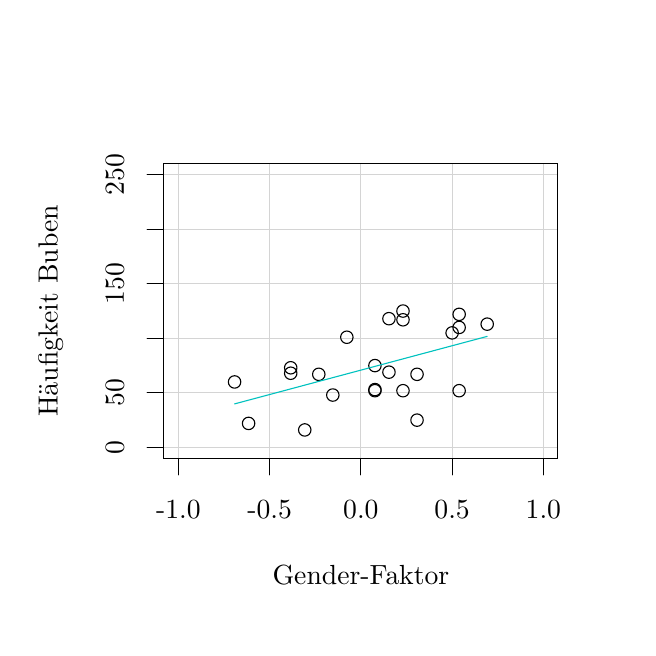
\begin{tikzpicture}[x=1pt,y=1pt]
\definecolor[named]{fillColor}{rgb}{1.00,1.00,1.00}
\path[use as bounding box,fill=fillColor,fill opacity=0.00] (0,0) rectangle (216.81,216.81);
\begin{scope}
\path[clip] (  0.00,  0.00) rectangle (216.81,216.81);
\definecolor[named]{drawColor}{rgb}{0.00,0.00,0.00}

\path[draw=drawColor,line width= 0.4pt,line join=round,line cap=round] ( 54.47, 61.20) -- (186.34, 61.20);

\path[draw=drawColor,line width= 0.4pt,line join=round,line cap=round] ( 54.47, 61.20) -- ( 54.47, 55.20);

\path[draw=drawColor,line width= 0.4pt,line join=round,line cap=round] ( 87.44, 61.20) -- ( 87.44, 55.20);

\path[draw=drawColor,line width= 0.4pt,line join=round,line cap=round] (120.41, 61.20) -- (120.41, 55.20);

\path[draw=drawColor,line width= 0.4pt,line join=round,line cap=round] (153.37, 61.20) -- (153.37, 55.20);

\path[draw=drawColor,line width= 0.4pt,line join=round,line cap=round] (186.34, 61.20) -- (186.34, 55.20);

\node[text=drawColor,anchor=base,inner sep=0pt, outer sep=0pt, scale=  1.00] at ( 54.47, 39.60) {-1.0};

\node[text=drawColor,anchor=base,inner sep=0pt, outer sep=0pt, scale=  1.00] at ( 87.44, 39.60) {-0.5};

\node[text=drawColor,anchor=base,inner sep=0pt, outer sep=0pt, scale=  1.00] at (120.41, 39.60) {0.0};

\node[text=drawColor,anchor=base,inner sep=0pt, outer sep=0pt, scale=  1.00] at (153.37, 39.60) {0.5};

\node[text=drawColor,anchor=base,inner sep=0pt, outer sep=0pt, scale=  1.00] at (186.34, 39.60) {1.0};

\path[draw=drawColor,line width= 0.4pt,line join=round,line cap=round] ( 49.20, 65.14) -- ( 49.20,163.67);

\path[draw=drawColor,line width= 0.4pt,line join=round,line cap=round] ( 49.20, 65.14) -- ( 43.20, 65.14);

\path[draw=drawColor,line width= 0.4pt,line join=round,line cap=round] ( 49.20, 84.85) -- ( 43.20, 84.85);

\path[draw=drawColor,line width= 0.4pt,line join=round,line cap=round] ( 49.20,104.55) -- ( 43.20,104.55);

\path[draw=drawColor,line width= 0.4pt,line join=round,line cap=round] ( 49.20,124.26) -- ( 43.20,124.26);

\path[draw=drawColor,line width= 0.4pt,line join=round,line cap=round] ( 49.20,143.96) -- ( 43.20,143.96);

\path[draw=drawColor,line width= 0.4pt,line join=round,line cap=round] ( 49.20,163.67) -- ( 43.20,163.67);

\node[text=drawColor,rotate= 90.00,anchor=base,inner sep=0pt, outer sep=0pt, scale=  1.00] at ( 34.80, 65.14) {0};

\node[text=drawColor,rotate= 90.00,anchor=base,inner sep=0pt, outer sep=0pt, scale=  1.00] at ( 34.80, 84.85) {50};

\node[text=drawColor,rotate= 90.00,anchor=base,inner sep=0pt, outer sep=0pt, scale=  1.00] at ( 34.80,124.26) {150};

\node[text=drawColor,rotate= 90.00,anchor=base,inner sep=0pt, outer sep=0pt, scale=  1.00] at ( 34.80,163.67) {250};

\path[draw=drawColor,line width= 0.4pt,line join=round,line cap=round] ( 49.20, 61.20) --
	(191.61, 61.20) --
	(191.61,167.61) --
	( 49.20,167.61) --
	( 49.20, 61.20);
\end{scope}
\begin{scope}
\path[clip] (  0.00,  0.00) rectangle (216.81,216.81);
\definecolor[named]{drawColor}{rgb}{0.00,0.00,0.00}

\node[text=drawColor,anchor=base,inner sep=0pt, outer sep=0pt, scale=  1.00] at (120.41, 15.60) {Gender-Faktor};

\node[text=drawColor,rotate= 90.00,anchor=base,inner sep=0pt, outer sep=0pt, scale=  1.00] at ( 10.80,114.41) {Häufigkeit Buben};
\end{scope}
\begin{scope}
\path[clip] ( 49.20, 61.20) rectangle (191.61,167.61);
\definecolor[named]{drawColor}{rgb}{0.83,0.83,0.83}

\path[draw=drawColor,line width= 0.4pt,line join=round,line cap=round] ( 54.47, 61.20) -- ( 54.47,167.61);

\path[draw=drawColor,line width= 0.4pt,line join=round,line cap=round] ( 87.44, 61.20) -- ( 87.44,167.61);

\path[draw=drawColor,line width= 0.4pt,line join=round,line cap=round] (120.41, 61.20) -- (120.41,167.61);

\path[draw=drawColor,line width= 0.4pt,line join=round,line cap=round] (153.37, 61.20) -- (153.37,167.61);

\path[draw=drawColor,line width= 0.4pt,line join=round,line cap=round] (186.34, 61.20) -- (186.34,167.61);

\path[draw=drawColor,line width= 0.4pt,line join=round,line cap=round] ( 49.20, 65.14) -- (191.61, 65.14);

\path[draw=drawColor,line width= 0.4pt,line join=round,line cap=round] ( 49.20, 84.85) -- (191.61, 84.85);

\path[draw=drawColor,line width= 0.4pt,line join=round,line cap=round] ( 49.20,104.55) -- (191.61,104.55);

\path[draw=drawColor,line width= 0.4pt,line join=round,line cap=round] ( 49.20,124.26) -- (191.61,124.26);

\path[draw=drawColor,line width= 0.4pt,line join=round,line cap=round] ( 49.20,143.96) -- (191.61,143.96);

\path[draw=drawColor,line width= 0.4pt,line join=round,line cap=round] ( 49.20,163.67) -- (191.61,163.67);
\end{scope}
\begin{scope}
\path[clip] (  0.00,  0.00) rectangle (216.81,216.81);
\definecolor[named]{drawColor}{rgb}{0.00,0.00,0.00}

\path[draw=drawColor,line width= 0.4pt,line join=round,line cap=round] ( 49.20, 61.20) --
	(191.61, 61.20) --
	(191.61,167.61) --
	( 49.20,167.61) --
	( 49.20, 61.20);
\end{scope}
\begin{scope}
\path[clip] ( 49.20, 61.20) rectangle (191.61,167.61);
\definecolor[named]{drawColor}{rgb}{0.00,0.00,0.00}

\path[draw=drawColor,line width= 0.4pt,line join=round,line cap=round] (155.91,108.49) circle (  2.25);

\path[draw=drawColor,line width= 0.4pt,line join=round,line cap=round] (130.55, 92.33) circle (  2.25);

\path[draw=drawColor,line width= 0.4pt,line join=round,line cap=round] (140.69, 91.55) circle (  2.25);

\path[draw=drawColor,line width= 0.4pt,line join=round,line cap=round] (135.62,111.25) circle (  2.25);

\path[draw=drawColor,line width= 0.4pt,line join=round,line cap=round] (135.62,114.41) circle (  2.25);

\path[draw=drawColor,line width= 0.4pt,line join=round,line cap=round] (155.91,113.22) circle (  2.25);

\path[draw=drawColor,line width= 0.4pt,line join=round,line cap=round] (153.37,106.52) circle (  2.25);

\path[draw=drawColor,line width= 0.4pt,line join=round,line cap=round] (135.62, 85.63) circle (  2.25);

\path[draw=drawColor,line width= 0.4pt,line join=round,line cap=round] (166.05,109.68) circle (  2.25);

\path[draw=drawColor,line width= 0.4pt,line join=round,line cap=round] (125.48, 85.63) circle (  2.25);

\path[draw=drawColor,line width= 0.4pt,line join=round,line cap=round] (115.33,104.95) circle (  2.25);

\path[draw=drawColor,line width= 0.4pt,line join=round,line cap=round] (105.19, 91.55) circle (  2.25);

\path[draw=drawColor,line width= 0.4pt,line join=round,line cap=round] (130.55,111.65) circle (  2.25);

\path[draw=drawColor,line width= 0.4pt,line join=round,line cap=round] (110.26, 84.06) circle (  2.25);

\path[draw=drawColor,line width= 0.4pt,line join=round,line cap=round] ( 95.05, 93.91) circle (  2.25);

\path[draw=drawColor,line width= 0.4pt,line join=round,line cap=round] ( 74.76, 88.79) circle (  2.25);

\path[draw=drawColor,line width= 0.4pt,line join=round,line cap=round] ( 95.05, 91.94) circle (  2.25);

\path[draw=drawColor,line width= 0.4pt,line join=round,line cap=round] (125.48, 94.70) circle (  2.25);

\path[draw=drawColor,line width= 0.4pt,line join=round,line cap=round] (155.91, 85.63) circle (  2.25);

\path[draw=drawColor,line width= 0.4pt,line join=round,line cap=round] (125.48, 86.03) circle (  2.25);

\path[draw=drawColor,line width= 0.4pt,line join=round,line cap=round] (140.69, 74.99) circle (  2.25);

\path[draw=drawColor,line width= 0.4pt,line join=round,line cap=round] (100.12, 71.45) circle (  2.25);

\path[draw=drawColor,line width= 0.4pt,line join=round,line cap=round] ( 79.83, 73.81) circle (  2.25);
\definecolor[named]{drawColor}{rgb}{0.00,0.76,0.75}

\path[draw=drawColor,line width= 0.4pt,line join=round,line cap=round] ( 74.76, 80.86) --
	(166.05,105.26);
\end{scope}
\end{tikzpicture}


\end{figure}

\subsection{Eigenschaftspaare}

Zur besseren Nachvollziehbarkeit des Genderfaktors sollen im Folgenden
drei der 13 Eigenschaftspaare etwas genauer vorgestellt werden, die
besonders aufgrund ihrer Signifikanz besonders aufgefallen sind.

\subsubsection{Unterwürfig/Dominant}

Unterwürfig ist eine Person besonders dann, wenn sie sich befehligen
lässt. Gehorsam zu sein und ohne viel Wiederstand seine eigene Position
aufzugeben sind weitere Beschreibungen dieser Eigenschaft. Dominante
Personen können hingegen ihren Willen gegenüber anderen durchsetzen.
Andere zu befehligen ist ein guter Indikator um dominante Charaktere zu
erkennen. Die Unterwerfung ist aus Sicht des Doing-Gender eine weibliche
Eigenschaft, während den Männern die Dominanz zugeschrieben wird.

Der w/m-Faktor korreliert dabei mit dieser Variabel sehr stark
($0{,}379; p=0{,}043$). Wir können daraus lesen, dass diese
Eigenschaften besonders klischeehaft in den gelesenen Kinderbüchern bei
den Hauptcharakteren verwendet wurden. Auffällig ist hier ebenfalls,
dass männliche Autoren dazu tendieren dominante Hauptprotagonisten zu
entwerfen ($r = 0{,}330; p=0{,}086$)

\subsubsection{Sicherheitsbedürftig/Abenteuerlustig}

Sicherheitsbedürftig zu sein äußert sich zumeist daran, dass eine
Persönlichkeit sehr zurückgezogen lebt und sehr überlegt handelt.
Zumeist umgeben sich sicherheitsbedürftige Menschen mit anderen Menschen
ihres persönlichen Vertrauens. Abenteuerlustige Personen gehen Risiken
ein und werfen sich der Gefahr entgegen. Dies tun sie meist ohne viel
darüber nachzudenken. Auch hier wird jede der Eigenschaften einem
Geschlecht stereotyp zugeteilt. Sicherheitsbedürftigkeit ist somit eine
weibliche Eigenschaft, während Männer abenteuerlustig sind.

Der w/m-Faktor korreliert dabei mit dieser Variabel sehr hoch
($0{,}384; p = 0{,}036$). Wir können daraus erkennen, dass dieses
Eigenschaftspaar besonders klischeehaft bei der Konstruktion von
Protagonisten in Kinderbüchern verwendet wird.

\subsubsection{Träumerisch/Realistisch}

Verträumte Entscheidungen sind oftmals optimistisch motiviert während
realistisches Denken starke rationale Gedankengänge verlangt. Oftmals
aus einer Laune heraus getroffen sind verträumte Entscheidungen spontan
aber auch mit Risiken verknüpft. Träumerisch wird aus Sichtweise des
Doing-Gender mit Femininität assozierte. Realistisch wird hier als
maskulines Attribut geführt.

Der w/m-Faktor korreliert mit dieser Variable am höchsten von allen
Eigenschaftspaaren (0,479; p= 0,01). Auch hier kann davon ausgegangen
werden, dass diese Eigenschaften besonders stereotyp verwendet werden.
Dabei sollte noch erklärt werden, dass alle anderen Eigenschaftspaare
gleich gepolt sind und zwar ebenfalls positiv korrelieren, das
Signifikanzniveau jedoch zu niedrig ist um eine klare Aussage zu
tätigen. Daher kann hier nur soweit interpretiert werden, dass keine
einzige Gender-Eigenschaft eine Tendenz zu einer nicht-klischeehaft
Verwendung vorweist.

\subsubsection{Beispiel Franz}

Wie man aus der Tabelle \ref{top30gender} entnehmen kann, werden die
Geschichten vom Franz bevorzugterweise von Mädchen gelesen und das
obwohl die Hauptfigur ein Bub ist. Der Gender-Faktor des lieben Franz
sieht jedoch ganz anders aus. Mit dem niedrigsten Wert aller 30
Hauptcharaktere stellt er den feministen Protagonisten dar und bietet
damit eine spannende Basis für eine inhaltsanalytische Untersuchung.

Situationsbeschreibung:

Franz spielt mit Sandra und Gabi Prinz und Prinzessin, wobei Sandra den
Prinzen spielt und Gabi - in die er sich verliebt hat - die Prinzessin.
Die beiden verlangen von ihm den Hofzwerg zu spielen und das obwohl er
sogern der Prinz wäre:
\blockcquote[30]{Noestlinger2010}{Als sie dann eines Tages wollte, dass der Franz den königlichen Hofzwerg spielte, da reichte es ihm! Und als sie dann noch erklärte, der Franz sollte sich deswegen nicht aufregen, denn für einen Prinzen sei er viel zu klein, da sah der Franz nur noch rot. Er warf der Sandra die Zipfelmütze, die er als Hofzwerg aufsetzen sollte, an den Kopf und lief nach Hause. Schluchzend warf er sich auf sein Bett und trommelte mit den Fäusten in sein Kissen.}
Die Geschichten vom Franz thematisieren auf humorvolle Weise die
Bewältigung des Alltags: Schulprobleme, die erste Liebe, Beziehungen,
Peinlichkeiten, Gefühle und Vieles mehr. Franz zeigt Emotionen und wirkt
oft so, als hätte er nicht viel Selbstbewusstsein. Anhand der drei
Eigenschaftspaare die vorgestellt wurden, kann man ihn als
unterwürfigen, sicherheitsbedürftigen und träumerischen Protagonisten
einordnen.

\subsection{Multiprotagonisten}

Leser und Leserinnen dieser Arbeit, die einige der hier untersuchten
Kinderbücher kennen oder gar selbst gelesen haben, wird aufgefallen
sein, dass nicht jedem der 30 Bücher ein klar definierter einzelner
Hauptcharakter zugeordnet werden kann. Durch eine starke Selektion von
ebenfalls wichtigen aber dennoch untergeordneten Charakteren, konnte
sich die Forschungsgruppe in den meisten Fällen auf einen einzelnen bzw.
den prägendsten Charakter einigen. Das dabei am heftigsten diskutierte
Opfer dieser Selektion ist Peter Pan, da die literarische Aufbereitung
des Textes von den meisten Verfilmungen abweicht und nicht Peter sondern
vielmehr Wendy im Mittelpunkt der Erzählungen steht. Besonders in den
Detektivgeschichten ist es zumeist nicht möglich einen Charakter als den
Hauptprotagonisten zu deklarieren, da diese fast ausschließlich aus
einem Team junger Detektive und Detektivinnen bestehen, die gleichwertig
nebeneinander agieren. Hier wurde das Prinzip des Multiprotagonisten
verwendet, der das Team als einen einzelnen Charakter erhebt. Um jedoch
einen Multiprotagonisten erstellen zu können, muss ein Kriterium erfüllt
werden: Die Charaktere müssen dasselbe Ziel haben. Zusammengefasst
handelt es sich bei Multiprotagonisten um eine Gruppe von Akteuren, die
jedoch in ihrer Gesamtheit ebenso als ein einziger Charakter verstanden
werden können, dessen komplexe Attribute - aufgrund der leichteren
Verständlichkeit für Kinder - in verschiedene Persönlichkeiten
aufgeteilt wurden. Nur wenn eine Gruppe als solches verstanden werden
kann, kann ein Multiprotagonist erstellt werden. Bei den zuvor genannten
Geschichten des Peter Pan wäre die Konstruktion eines solchen
Multiprotagonisten beispielsweise nicht möglich gewesen, da sowohl Wendy
wie auch Peter Pan als eigenständige Charaktere begriffen werden müssen
und über kein gemeinsames Ziel verfügen. Zum leichteren Verständnis wird
hier ein Beispiel eines solchen Multiprotagonisten genannt und erklärt:

\subsubsection{Beispiel: Tom Turbo}

Das Dreiergespann Tom Turbo, Karo und Klaro können als ideales Beispiel
für einen Multiprotagonisten fungieren. Tom Turbo ist das tollste
Fahrrad der Welt mit zahlreichen Tricks, die auf der Verbrecherjagt von
Nutzen sein können. Seine Detektivkollegen Karo und Klaro sind ein
Geschwisterpaar. Karo ist ein taffes kleines Mädchen, dass sich ohne
viel scheu in ein Abenteuer wirft, genauso wie ihr Bruder Klaro der
oftmals sogar etwas nachdenklicher wirkt als seine Schwester. Sie
trennen sich während der Bewältiung ihrer Abenteur nie, wenn nicht einer
der drei das Opfer der Geschichte ist (Beispiel Entführung). Alle drei
gemeinsam haben, dasselbe Ziel und sind zumeist der gleichen Meinung.
Entsteht einmal ein Disput zwischen den beiden Geschwistern ähneln diese
einer Abwägung von Pros und Contras, die auch eine einzelne Person
gedanklich abarbeiten würde, stecke sie in einer ähnlichen Situation.
\parencite{Leope2008}

\section{Merkmale des inhaltlichen Aufbaus}

Aus dem Wissen, dass Buben und Mädchen unterschiedliche Lesepräferenzen
aufweisen, ergibt sich die Frage, worin sie sich unterscheiden. Es ist
bekannt, dass Buben verstärkt auf Sachbücher -- die in unserer Erhebung
bewusst auf Grund der fehlenden Darstellungen von Protagonisten nicht
erhoben wurden - ansprechen, Mädchen hingegen tendieren zu Büchern die
eine Geschichte erzählen. In unserer Erhebung haben wir ausschließlich
Bücher erhoben, die aus dieser Unterscheidung von Mädchen favorisiert
werden sollten. Dennoch konnte hier kein nennenswerter Unterschied in
der Menge des Gelesenen festgestellt werden, was es uns ermöglicht, die
unterschiedlichen Lesepräferenzen auf eine andere Form hin zu
untersuchen. Hierbei wurde analysiert, ob es sich bei den Büchern um
Abenteuer- oder Alltagsgeschichten handelt (siehe Tabelle \ref{genre}).

      
      \ctable[
      %  cap    = ,
        caption = {Inhaltliche Merkmale von Geschichten},
        label   = genre ,
        pos   = htp,
      %  width    = \textwidth
      ]{lccccc}{}{                  
      \FL \small Bücher &  
      \multicolumn{1}{c}{\small Phant} & 
      \multicolumn{1}{c}{\small Grow} & 
      \multicolumn{1}{c}{\small Mono} & 
      \multicolumn{1}{c}{ \small Quest} & 
      \multicolumn{1}{c}{ \small Abenteuer}
      \ML Die wilden Fußballkerle &  &    &     &     & Alltag
      \NN Tiger-Team          &     &     &     & x   & Abenteuer
      \NN Knickerbockerbande  &     &     &     & x   & Abenteuer
      \NN Gregs Tagebuch      &     &     & x   &     & Alltag
      \NN Harry Potter        & x   & x   &     & x   & Abenteuer
      \NN Die drei ???        &     &     &     & x   & Abenteuer
      \NN Das magische Baumhaus & x &     &     &     & Abenteuer
      \NN Der kleine Ritter Trenk & x &   &     & x   & Abenteuer
      \NN Tom Turbo           & x   &     &     & x   & Abenteuer
      \NN Der kleine Drache Kokosnuss & x & &   & x   & Abenteuer
      \NN Der Räuber Hotzenplotz & x &    &     & x   & Abenteuer
      \NN Sams                & x   &     &     &     & Alltag
      \NN Fünf Freunde        &     &     &     & x   & Abenteuer
      \NN Die Olchis          & x   &     &     &     & Alltag
      \NN Der Grüffelo        & x   &     &     &     & Alltag
      \NN Die Geggis          & x   & x   & x   &     & Abenteuer
      \NN Peter Pan           & x   & x   & x   &     & Abenteuer
      \NN Der Regenbogenfisch & x   & x   & x   &     & Alltag
      \NN Baumhausgeschichten &     &     &     &     & Alltag
      \NN Geschichten von Franz &   & x   & x   &     & Alltag
      \NN Pinocchio           & x   & x   &     &     & Abenteuer
      \NN Das kleine Wutmonster & x & x   &     &     & Alltag
      \NN Der kleine Eisbär   & x   & x   &     &     & Abenteuer
      \NN Pipi Langstrumpf    & x   &     &     &     & Alltag
      \NN Die kleine Hexe     & x   &     &     &     & Alltag
      \NN Hexe Lilli          & x   &     &     & x   & Alltag
      \NN Die wilden Hühner   &     &     &     & x   & Alltag
      \NN Mini                &     & x   & x   &     & Alltag
      \NN Conni               &     & x   &     &     & Alltag
      \NN Prinzessin Lillifee & x   &     &     & x   & Abenteuer 
      \LL
      }
      

\subsection{Alltagsgeschichten}

Alltagsgeschichten spielen in einem dem Hauptprotagonisten vertrauten
Umfeld. Bei kindlichen Protagonisten handelt es sich zumeist um die
familiäre und/oder schulische Umgebung. Es werden Themen und
Problematiken angesprochen, die im realen Leben der Leser und Leserinnen
mit großer Wahrscheinlichkeit vorkommen können. Beispiele dafür sind
Beziehungsprobleme mit Freunden, Eltern oder Lehrern, aber auch
Leistungsdruck in der Schule, Erlebnisse auf Klassenfahrten, Urlaube
oder der Tod von Haustieren.

\subsubsection{Beispiel: Hexe Lilli}

``Das ist Lilli, die Hauptperson unserer Geschichte. Sie ist ungefähr so
alt wie du und sieht aus wie ein gewöhnliches Kind.''
\parencite[][6]{KNISTER1999} Bereits dieser Satz, mit dem die Erzählung
beginnt, verrät viel darüber wie versucht wird, den Leser/ die Leserin
in die Geschichte zu integrieren, was in späterer Folge nicht schwer
fällt, da Lilli Situationen durchlebt, die wohl keinem gänzlich
unbekannt sind. Zankerein mit dem kleinen Bruder, sowie Unverständnis
über die Einstellungen der Eltern gehören wohl zum vielfältigen
Kinderalltag.

Situationsbeschreibung: Der Schulrat besucht an diesem Tag die Klasse
von Lilli und möchte den Unterricht von Frau Grach der Klassenlehrerin
inspizieren. Lilli möchte der Frau Lehrerin gerne helfen einen guten
Eindruck zu hinterlasssen, doch der Herr Schulrat taucht natürlich genau
im falschen Moment auf als das totale Chaos in der Klasse herrscht.
\blockcquote[47]{KNISTER1999}{\enquote{Auweia}, flüstert Lilli. So war das nicht gedacht! Hier muss sie schnell eingreifen bevor der Schulrat gleich zu Anfang einen schlechten Eindruck bekommt.}
Lilli ist tatkräftig und dominant aber zugleich auch hilfsbereit und
großherzig. Sie bietet aus Sicht des Doing-Gender einen Mix an
Eigenschaften, der sich auch im Wert der Gendertabelle (siehe
Tabelle\ldots{}) widerspiegelt. Lilli wird sehr klar bevorzugt von
Mädchen gelesen und zeigt, wie Mädchen ebenfalls mit maskulinen
Genderatributen dargestellt werden. Sie ist ein Paradebeispiel dafür,
dass Mädchen mit beiden Genderrollen konfrontiert werden, was Buben
gemeinhin noch verwehrt wird.

\subsection{Abenteuergeschichten}

Abenteuergeschichten sind das Gegenstück zu Alltagsgeschichten. Dabei
durchlebt der Hauptprotagonist ein wahrscheinlich einzigartiges
Erlebnis, das zumeist mit großen Risiken und Gefahren verbunden ist. Der
Protagonist ist dabei zumeist gezwungen sein gewohntes Umfeld zu
verlassen und sich in völlig fremden oft auch unrealistischen
Situationen zurechtzufinden. Beispiele hierfür wären die Suche nach
einem verschollenen Schatz, das Tätigen einer gefährlichen und
ungewissen Reise, das Kämpfen mit bösen Mächten wie Ganoven oder Drachen
usw.

\subsubsection{Beispiel: Harry Potter}

Harry ist ein schmächtiger Junge, der bei der Familie seiner Tante lebt,
da seine Eltern gestorben sind. Das allerdings nur so lange bis er
erfährt, das er ein Zauberer ist und auf die Zauberschule kommt. Dort
angekommen erlebt er ein Abenteuer nach dem anderen. Diese Gipfeln in
einem großen und brutalen Show-Down im Kampf gegen den Mörder seiner
Eltern. \parencite{Rowling1998}

Harry Potter hat viele Attribute die feminin deklariert sind, so ist er
beispielsweise großherzig und emotional, manchmal sogar etwas
träumerisch, aber auch mutig und aktiv. Er ist teilweise sehr dominant
und hält sich nicht an Regeln. Diese Attribute lassen den Genderwert
leicht ins maskuline wandern. Sein Genderwert ist beispielsweise jenem
von Hexe Lilli nicht unähnlich, die Bücher werden schließlich auch von
vielen Mädchen gerne gelesen, jedoch tendenziel eher von Jungen. Harry
Potter ist ein passendes Beispiel dafür, dass Jungen männliche
Protagonisten, vor allem aber auch Abenteuergeschichten favorisieren.

Wie wir auf Tabelle \ref{genre}. erkennen lesen Buben verstärkt
Abenteuergeschichten während Mädchen einen viel höhere Anzahl an
Alltagsgeschichten in ihrer Lesepräferenz vorweisen. Dies kann auch mit
einer Korrelation von 0,314 (Sig. 0,091) statistisch festgehalten
werden. Auch hier finden wir dasselbe Bild, dass Mädchen in beiden
Ausprägungen zu finden sind, Buben hingegen nur sehr wenige
Alltagsgeschichten lesen.

Doch hat diese unterschiedliche Präferenz eine Auswirkung auf die
unterschiedliche Entwicklung von Geschlechterausprägungen? Diese Frage
kann anhand der erhobenen Daten nicht beantwortet werden und dennoch
kann sie dazu nutzen eine weitere Frage aufzuwerfen, die einen
Anhaltspunkt für die Beantwortung liefern kann. Aus unserer Erhebung zur
Darstellung von Gendermerkmalen (siehe Genderfaktor) wissen wir, dass
gewisse Eigenschaften als besonders maskulin oder feminin empfunden
werden. Wir haben uns daher gefragt, ob es denn Merkmale im Inhalt und
Aufbau von Kinderbüchern geben könnte, die die Ausprägung solcher
Eigenschaften unterstützen. Da die Ergebnisse für Jungen viel
einseitiger ausgefallen sind, kann die Frage auch wie folgt formuliert
werden. Haben beispielsweise Abenteuergeschichten bestimmte Merkmale,
mit denen Buben verstärkt konfrontiert werden und können sie als ein
möglicher Faktor zur Entwicklung \emph{maskuliner} Eigenschaften
beitragen? Oder: Fehlen durch das sparsame Lesen von Alltagsgeschichten
bestimmte Merkmale, die eine femininere Entwicklung verhindern?

Folgende vier Kriterien wurden erhoben, bei denen von einem Einfluss auf
die Geschlechterrollenentwicklung ausgegangen wurde:

\subsubsection{Quest}

Verläuft die Geschichte des Buches auf ein bestimmtes Ziel hin, das
erreicht werden soll? Erfordert das Erreichen des Zieles das Lösen von
Aufgaben bzw. Rätseln? Besonders Kriminal- und Detektivgeschichten sind
mit einem obersten Ziel verknüpft, dass erreicht werden soll. Auf dem
Weg bis zur Lösung stellen sich dem Protagonisten Stolpersteine in den
Weg, die zuerst entfernt werden müssen. Dies braucht oft rationales
Denken, Mut, aktives Handeln oftmals auch körperliche Stärke und
Aggression. All diese Attribute werden im Sinne des Doing-Gender als
maskuline Eigenschaften wahrgenommen und könnten daher eine spezifische
Geschlechterrollenentwicklung miterklären. Es ist daher wenig
überraschend, dass die Präsenz von Quests in enger Verbindung mit
Abenteuergeschichten steht. Bei einer hochsignifikanten Korrelation von
0,517 kann daher auch eine Verknüpfung mit einem verstärkten Vorkommen
in den Büchern mit männlicher Lesepräferenz ausgegangen werden.

\paragraph{Beispiel \emph{Die Knickerbockerbande}}

Die Knickerbockerbande besteht aus Lilo, Axel, Dominik und Poppi, die in
jedem Band neue \emph{Rätsel} lösen. Dabei kann es vorkommen, dass sie
etwa im Urlaub auf mysteriöse Fälle stoßen, die sie dann meist zu viert
aufklären. Die Geschichten sind spannend, die vier geraten öfter in
Gefahr oder in die Hände von Verbrechern, aus denen sie sich aber mit
List und Geschick wieder befreien. Dies ist ein eindeutiger Indikator
für das Merkmal des Quests. Die Hauptfiguren haben unterschiedliche
Qualitäten, können aber als ein Multiprotagonist verstanden werden. Auch
das Verhalten untereinander ist sehr hilfsbereit, sie sind verlässlich
und sie alle vereint dasselbe Hobby, nennen wir es ``Dedektiv spielen'',
worauf sie sich auch in ihrer Freizeit vorbereiten und trainieren, wie
man sich zum Beispiel anschleicht oder besonders schnell ist. Die
Geschichten wirken anfangs mysteriös, was auch die Titel wiedergeben,
die manchmal gruselige und surreale Situationen zu versprechen scheinen,
die sich dann aber immer als menschengemacht herausstellen.
\blockcquote[117]{Brezina2010}{Die Männer in den roten Mänteln lagen kraftlos am Boden. \textelp{}  Axel waren sofort die kleinen roten Federbüschel aufgefallen, die ihnen seitlich aus dem Hals ragten. Sie dienten einer kleinen Nadel als Stabilisator. Solche Nadeln wurden aus Blasrohren abgefeuert. Axel erinnerte sich, etwas im Fernsehen darüber gesehen zu haben.}
Die Protagonisten agieren sehr rational. Sie können Situationen gut
einschätzen und verknüpfen das Wissen aus anderen Informationsquellen
mit dem Erlebten. Diese Eigenschaft hilft ihnen dabei die Rätsel zu
lösen und ihr Ziel zu erreichen.

\subsubsection{Phantastische Elemente}

Kommen in den Büchern Figuren, Orte oder Handlungen vor, die in der
Realität nicht vorkommen? Beispiele: Einhörner, sprechende Tiere,
fliegende Menschen, Zauberer, fremde Welten, uvm. Phantastische Elemente
könnten einen Hang zum träumerischen, irrationalen Denken fördern,
welches aus der Sicht des Doing-Genders feminine Attribute wären. Doch
Abenteuergeschichten sind natürlich gespickt mit unmöglichen
Situationen. Oftmals bekämpfen Charaktere Monster und Gespenster. Daher
tendieren die Zahlen dazu, das Vorkommen von phantastischen Elementen
den Abenteuerbüchern zuzuschreiben. Das niedrige Signifikanzniveau lässt
hier jedoch keine genaue Aussage zu. Es kann auch kein Zusammenhang mit
dem w/m-Faktor gefunden werden. Dieses inhaltliche Merkmal scheint in
beiden Geschlechtsgruppen annähernd gleich oft verwendet zu werden und
kann daher keine Annäherung zur Erklärung von Geschlechtsrollenbildung
liefern.

\subsubsection{Innerer Monolog}

Welche Rolle spielt die Gedankenwelt des Hauptprotagonisten? Wie stark
reflektiert er seine Entscheidungen vor und/oder nach dem Handeln? Wie
intensiv wird sie dem Leser/der Leserin vermittelt? Mädchen gelten als
passiver und introvertierter als ihre männlichen Altersgenossen und
haben aus Sicht des Doing-Gender ein größeres Einfühlungsvermögen als
Jungen. All dies wären Indizien den Inneren Monolog als ein Merkmal zu
deklarieren, das Jungen fehlen könnte eine feminine Seite zu entwickeln.
Und tatsächlich tendieren die Zahlen unserer Ergebnisse dazu einen
Zusammenhang von Alltagsgeschichten und Innerem Monolog zu bescheinigen.
Auch hier ist jedoch das Signifikanzniveau zu niedrig um fixe Aussagen
zu tätigen. Auffällig ist, dass das Merkmal des Inneren Monologs negativ
mit dem Merkmal Quests korreliert ($r= -0{,}333; p=0{,}083$). Das
bedeutet, dass das kombinierte Vorkommen dieser beiden Merkmale äußerst
selten anzutreffen ist.

\paragraph{Beispiel Mini}

In den Mini-Büchern geht es darum den frühen Alltag eines Kindes zu
bewältigen und persönliche Konflikte auf sehr humorvolle Art aus Minis
Sicht wiederzugeben.

Mini ist schon sehr groß für ihr Alter und gleichzeitig sehr dünn,
weshalb ihr auch alle möglichen Spitznamen gegeben werden, was sie
kränkt. Der Schule blickt sie mit gemischten Gefühlen entgegen,
gleichzeitig freut sie sich schon drauf, hat aber auch Angst in die
falsche Schule zu kommen, von der die falschen Lehrerin unterrichtet zu
werden oder vor den fremden Kindern, die sie wieder hänseln könnten.
Dies zeigt wie viel sie reflektiert und über mögliche Situationen und
Folgen nachdenkt. Als Beispiel kann hier der Gedankengang genannt
werden, der zeigt wie erleichtert sie darüber ist, dass sie nicht die
größte in ihrer Klasse ist:
\blockcquote[61]{Noestlinger2011}{Und die Mini fing vor lauter Staunen zu schielen an. \textelp{} Warum die Mini so erstaunt und verblüfft war? Weil sie garantiert nicht das größte Kind ihrer Klasse war! Ein Bub und ein Mädchen waren noch ein bisschen größer als die Mini, 2 Buben und 2 Mädchen waren genauso groß wie die Mini. Die Mini dachte: \enquote{Wenn es unter zwanzig Kindern sieben \emph{lange Latten} gibt, dann ist ja die Überlänge direkt normal!}}

\subsubsection{Growing-Up:}

Verändert sich im Verlauf der Geschichte die Persönlichkeit des
Hauptprotagonisten? Durchläuft er einen Reifeprozess? Erhebt das Buch
den Anspruch eine pädagogische Nachricht zu vermitteln, hingerichtet auf
eine positive Sozialisierung? Mädchen gelter oftmals im Vergleich zu den
gleichaltrigen Jungen als sozial weiter entwickelt. Dieser Vorsprung in
der Entwicklung könnte zum Teil durch eine vermehrte Konfrontation mit
pädagogisch motivierter Literatur mitbegründet sein. Es kann hier jedoch
kein Zusammenhang festgestellt werden. Lediglich eine starke
signifikante Korrelation mit dem Merkmal des Inneren Monologs kann hier
festgestellt werden, sowie eine stark signifikante negative Korrelation
mit dem Merkmal Quest, wie auch schon beim Merkmal des Inneren Monologs.

Die Untersuchung der vier inhaltlichen Merkmale von Alltags- und
Abenteuergeschichten konnte vor allem zeigen, dass eine Analyse anhand
von 30 Büchern keine wirklichen aussagekräftigen Ergebnisse liefern kann
und hier eine große eigenständige Untersuchung notwendig wäre um etwaige
Zusammenhänge zwischen inhaltlichen Merkmalen und der Ausprägungen von
geschlechterspezifischen Eigenschaftsmerkmalen notwendig wäre. Somit
bleibt hier als einziges aussagekräftiges Ergebnis nur die Erkenntnis,
dass sich die Buben bei ihrer Lesepräferenz vor allem auf
Abenteuergeschichten konzentrieren, Mädchen hingegen auch
Alltagsgeschichten lesen. Als kleiner Hoffnungsschimmer am Firmament ist
die Untersuchung des Merkmals Quests zu sehen, die gezeigt hat, dass das
Vorkommen eines Merkmals mit bestimmten Eigenschaften die als maskulin
deklariert sind in Verbindung gebracht werden und eine größere
Untersuchung womöglich aussagekräftigere Ergebnisse liefern könnte.

\section{Fazit und Verknüpfung mit der Theorie}

Als großer Triumpf dieses Kapitels ist die Untersuchung der
Gendermerkmale von Hauptprotagonisten in Kinderbüchern zu sehen. Sie hat
uns gezeigt, dass Buben vor allem über maskuline Charaktere lesen,
Mädchen zu weiblichen tendieren aber mit beiden konfrontiert werden.
Weiterhin werden manche stereotype Eigenschaften bestimmten
Geschlechtern zugeschrieben und verhindern damit den Prozess des
Gender-Mainstreaming. Das soziale Geschlecht kann hier ergänzend zum
Geschlecht gesehen werden um das Doing-Gender von Kinderbuchcharakteren
zu erklären. Die Regression zeigt uns, dass die Wahrscheinlichkeit einer
Erklärung steigt, wenn beide Faktoren miteinander kombiniert werden.($r$
bei Geschlecht: 0.58; bei Gender: 0.19; Kombiniert: 0.66).

Der Versuch dieses Ergebnis mit Theorie zu verknüpfen kann zu
provokanten Aussagen führen, die hier nur genannt werden um etwaige
Untersuchungen in der Zukunft motivieren. So kann etwa unser Wissen,
dass Mädchen und Buben unterschiedliche Bücher lesen mit der Theorie
verknüpft werden, dass das Verhalten von Protagonisten in Büchern auf
deren Leser abfärbt und somit Verhalten reproduziert. Diese Verknüpfung
würde aus Sicht der Ergebnisse dieser Untersuchung wie folgt zu
interpretieren sein: Wenn Buben verstärkt mit maskulinen Protagonisten
konfrontiert werden, könnte diese Einseitigkeit zu einer Stabilisierung
von stereotypen Geschlechterrollen führen. Bei Mädchen hingegen sagen
uns die Ergebnisse, dass sie inzwischen mit vielfältigeren Eigenschaften
und Handlungsalternativen konfrontiert werden und daher im Sinne des
Gender-Mainstreamings eine größere Chance haben, bestehende stereotype
Rollenbilder zu brechen und neu zu gestalten.

\chapter{Merkmale die das Leseverhalten erklären}

Drei Merkmale eines Kinderbuchs reichen aus, um das Verhältnis von
Leserinnen zu Lesern bei einem Kinderbuch bestimmen zu können: das
\emph{Geschlecht der Titelfigur}, die \emph{Helligkeit} und die
\emph{Anzahl der Seiten}. Die Genauigkeit eines linearen Modells mit
diesen drei Merkmalen ist mit einem korrigierten Bestimmtheitsmaß von
$0{,}82$ sehr genau. Wobei das Vorhandensein einer weiblichen Namens im
Titel am meisten zu dem Modell beiträgt ($\beta=-0{,}77$). Danach kommt
die Helligkeit des Covers ($\beta=0{,}29$). Die Anzahl der Seiten dient
dann nur noch zu Verfeinerung ($\beta=0{,}19$). Stellte man eigene
Modelle für das Geschlecht der Titelfigur sowie für die Coverhelligkeit
auf sieht man, dass Beide auch alleine noch einen beachtlichen Teil
erklären. (Siehe Tabelle~\ref{wmmodel})

All diese Merkmale können von Kindern ohne Probleme und ohne dass sie
das Buch aufmachen müssen wahrgenommen werden. Unsere beiden Fragen, ob
Merkmale des Buchs das Verhältnis von Leserinnen zu Lesern erklären und
ob sie das ohne das Buch zu öffnen können, können wir eindeutig mit
\emph{ja} beantworten. Steht im Titel ein weiblicher Name, ist das Buch
noch dazu sehr hell und obendrein auch noch dünn. Dann ist die
Wahrscheinlichkeit sehr hoch, dass das Buch viel mehr Mädchen als Buben
gelesen haben. Ist das Buch dunkel, dick und kommt auch noch ein
männlicher Name im Titel vor, ist es wahrscheinlicher, dass mehr Buben
als Mädchen das Buch gelesen haben.

      
      \ctable[
      %  cap    = ,
        caption = {Lineare Modelle die den w/m-Faktor erklären},
        label   = wmmodel ,
        pos   = htp,
      %  width    = \textwidth
      ]{lD{,}{,}{2}D{,}{,}{2}D{,}{,}{2}}{
        % \tnote[.]{< 0,1}
        % \tnote[*]{< 0,05}
        % \tnote[**]{< 0,01}
        % \tnote[***]{< 0,001}
      }{                  
      \FL 
      \small   &  
      \multicolumn{1}{c}{\small Modell 1} & 
      \multicolumn{1}{c}{\small Modell 2} & 
      \multicolumn{1}{c}{\small Modell 3}
      \ML Geschlecht Titelfigur (unbestimmt)    & 0,06      & 0,02      &
      \NN Geschlecht Titelfigur (weiblich)      & -0,77\tmark[***]     & -0,82\tmark[***]     & 
      \NN Geschlecht Titelfigur (männlich)      & \multicolumn{1}{c}{ref.}      & \multicolumn{1}{c}{ref.}      & 
      \NN Coverhelligkeit                       & -0,29\tmark[**]     &           & -0,46\tmark[**]
      \NN Seitenanzahl                          & 0,19\tmark[*]      &           & 
      \ML Korrigiertes $R^2$                    & 0,82\tmark[***]      & 0,69\tmark[***]      & 0,18\tmark[**]  
      \LL \multicolumn{4}{l}{\footnotesize  $^*p<0{,}05, ^{**}p<0{,}01, ^{***}p<0{,}001$}
      }
      

\section{Für Mädchen und Buben sind unterschiedliche Merkmale
ausschlaggebend}

Dies heißt jedoch nicht, dass die drei Merkmale auf Mädchen und Buben
denselben Einfluss haben. Die Wahrscheinlichkeit, dass Mädchen oder
Buben ein Buch lesen, hängt mit unterschiedlichen Merkmalen von Büchern
zusammen. Dafür, dass ein Buch hauptsächlich von Mädchen gelesen wird,
ist es wichtig, dass das Buch von einer Frau geschrieben wurde
($R^2 \scriptstyle kor.\textstyle =0{,}19; p=0{,}04$), wiederum, dass
die Figur im Titel weiblich ist
($R^{2}\scriptstyle kor.\textstyle =0{,}18; p=0{,}03$) und dass wenige
Figuren am Cover ($r=-0{,}37; p=0{,}4$) sichtbar sind. Insgesamt hat das
Modell mit diesen drei Merkmalen ein korrigiertes Bestimmtheitsmaß von
$0{,}33$ ($p=0{,}02$). Die Helligkeit und die Anzahl der Seiten ist für
die Anzahl der Mädchen die ein Buch lesen irrelevant.

Diese Merkmale sind für die Häufigkeit bei den Buben natürlich um so
wichtiger. (Helligkeit: $R^2 \scriptstyle kor.\textstyle =0{,}25$;
Seiten: $R^2 \scriptstyle kor.\textstyle =0{,}16$; $p=0{,}01$) Das lässt
auch darauf schließen, dass grundsätzlich das Leseverhalten von Buben
für das Verhältnis zwischen Mädchen und Buben relevanter ist. Und
tatsächlich ist die Korrelation zwischen der Häufigkeit der Nennungen
pro Buch bei den Buben und dem Verhältnis der Nennungen zwischen Mädchen
und Buben mit $0{,}70$ größer als zwischen den Mädchen und dem
Verhältnis, dass nur eine Korrelation von $-0{,}41$ aufweist. Da die
Nennungen der Buben für unser Verhältnis so wichtig sind, fangen wir
hier mit einer detaillierteren Analyse der Merkmale an.

\section{Das Geschlecht der Titelfigur}

Der erste Einflussfaktor ist das Geschlecht der Figur, die im Titel
genannt wird. Das ist in den meisten Fällen auch die Hauptfigur, also
die Figur mit der sich die Leserin oder der Leser am wahrscheinlichsten
identifiziert. Nur bei wenigen Geschichten ist die Figur, die am Titel
erwähnt wird, nicht die eigentliche Protagonistin bzw. der eigentliche
Protagonist. Auch wenn die Hauptfigur eine andere ist, heißt das noch
immer nicht, dass sich auch das Geschlecht unterscheidet. Zum Beispiel
ist in \emph{der Räuber Hotzenplotz} die Hauptfigur der Kasperl, aber
beide sind männlich. In \emph{Grüffelo} ist die Hauptfigur eine Maus und
beide sind \emph{neutral}. In unseren 30 meist genannten Büchern bleibt
nur ein Buch übrig, bei denen sich das Geschlecht der Titelfigur und der
Hauptfigur unterscheiden und hier handelt es sich um einen Streitfall.
Gemeint ist \emph{Peter Pan}, bei dem, im Original, Wendy die
Protagonistin ist. Jedoch ist bei vielen Adaptionen der Fokus ganz zu
Peter gewandert. Eine andere Möglichkeit einer Differenz zwischen den
beiden Merkmalen ist, dass das Geschlecht der Hauptfigur nicht vorkommt
oder nicht eindeutig bestimmbar ist.

Das Geschlecht der Hauptfigur ist ein Merkmal, über das die Autorin oder
der Autor die völlige Kontrolle haben. Das Geschlecht der Hauptfigur
entsteht meist ganz am Anfang und hat insgesamt gesehen den größten
Erklärungswert für das Gesamt-Modell und ist für Mädchen und Buben
relevant.

\section{Buben lesen keine hellen Bücher}

Das nächste wichtige Merkmal ist die Cover-Helligkeit eines Buchs.
Dieses Merkmal hat bei Buben immerhin einen gleich großen Erklärungswert
wie das Geschlecht der Titelfigur. Die Entstehung dieses Merkmals ist
jedoch schon nicht mehr direkt mit der Autorin oder dem Autor zu
verbinden. Das Cover wird zu einem Zeitpunkt, an dem die Geschichte
schon längst an einen Verlag verkauft worden ist, gestaltet. Es kann
auch vorkommen, dass das Cover bei neueren Fassungen komplett anders
gestaltet wurde. Der Verlag hat die Aufgabe die Geschichte an den
Endkunden zu verkaufen. Das heißt, es ist seine Aufgabe, Kindern, deren
Eltern und weiteren potenziellen Käufern die Entscheidung zu
erleichtern.

Wir vermuten, dass die Verlage herausgefunden haben, dass dunkle
\emph{coole} Bücher Buben eher ansprechen als lieblich helle, rosa
Bücher. Zusätlich muss der Verlag eine Entscheidung treffen, für wen die
Geschichte gedacht ist. Der Verlag hat für diese Zeit mehr Ressourcen
als der Endkunde. Hier werden Inhalte eines Buches von den dafür
zuständigen Personen im Cover ausgedrückt und gewissermaßen
\emph{übersetzt}. Dabei wirkt es nicht überraschend, dass sie sich an,
in der Gesellschaft verfestigten Geschlechterrollenbildern orientieren.
Tatsächlich hat der \emph{Gender-Faktor} auf die Helligkeit den größten
Einfluss ($r=-0{,}51$). Gemeinsam mit dem Geschlecht der Hauptfigur
lässt sich die Helligkeit schon recht gut voraussagen
($R^2 \scriptstyle kor.\textstyle =0{,}24; p=0{,}02$). So ist die
Helligkeit ein gutes \emph{Transportmittel} um den Gender-Faktor
ankommen zu
lassen.\footnote{Wir gehen davon aus, dass weitere Merkmale des Covers, die wir nicht operationalisiert haben, wie die Form der Darstellung oder die Komplexität des Bildes noch einen wesentlichen Anteil zur Übersetzung des Genderfaktor beitragen.}

Nicht übersehen darf man, dass nur das Leseverhalten von Buben von der
Helligkeit beeinflusst wird. Bei den Mädchen kann kein Zusammenhang mit
der Helligkeit nachgewiesen werden. Das heißt Mädchen lesen genauso
helle wie dunkle Bücher. Buben meiden jedoch helle Bücher. Das zeigt,
dass Buben es eher vermeiden mädchenhafte Literatur zu konsumieren,
während der Spielraum der Mädchen hier weniger eingeschränkt wird.

\section{Buben bevorzugen Bücher für Ältere}

Ein weiterer Einfluss auf das Leseverhalten, speziell von Buben, ist die
Dicke eines Buchs beziehungsweise das eng damit zusammenhängende
empfohlene Alter. Und zwar steigt mit der Dicke der Bücher auch die
Anzahl der männlichen Leser. Auf den ersten Blick widerspricht dieser
Fakt den Ergebnissen der Lesesozialisationsforschung, in der Buben meist
als \emph{Lesemuffel} dargestellt werden. Vor allem weil das
Leseverhalten von Mädchen dadurch wiederum nicht nachweisbar beeinflusst
wird. Weiters kann man hier auch nicht klar zu sagen welches Merkmal,
Alter oder Dicke, eigentlich wirksam ist.

Um das Wirken des Merkmalpaares haben wir zwei Vermutungen. Die erste
bezieht sich darauf, dass Mädchen früher zu lesen beginnen. Wir haben
die Kinder gefragt, welche Bücher sie gelesen haben. Die befragten
Kinder waren zwischen 8 und 10 Jahren und es ist durchaus vorstellbar,
dass die Mädchen früher zum Lesen von \emph{Geschichten-Büchern}
anfangen. Das heißt, dass sie davor weniger oder andere von uns nicht
untersuchte Bücher, wie die bei den Buben sehr beliebten Sachbücher,
lesen. Die zweite Vermutung bezieht sich auf den \emph{Coolness-Faktor}.
Das heißt, das es für Buben wichtiger ist \emph{cool} zu sein. So kann
sich von unserer Forschungsgruppe ein männliches Mitglied noch sehr gut
erinnern, dass das empfohlene Alter hinten auf den Büchern, für ihn,
gerade im Alter der Untersuchten, sehr wichtig war.

\section{Der Einfluss des Geschlechts der Autorin/des Autors ist zu
vernachlässigen}

Wenden wir uns wieder dem Modell, dass die Häufigkeiten der Mädchen
erklären soll, zu. Davon haben wir das für die Mädchen zweitwichtigste
Merkmal, das Geschlecht der Titelfigur, schon analysiert. Jedoch kommt
bei den Mädchen ein weiteres \emph{Geschlechts-Merkmal} hinzu. Das
Geschlecht der Autorin/des Autors. Bei diesem Oberflächenmerkmal ist für
die Buben kein Zusammenhang nachweisbar.

Aber auch die Erklärungskraft bei den Mädchen ist nicht überzubewerten,
da sie zu einem sehr großen Teil aus einem sehr gewichtigen
\emph{Ausreißer} besteht. Der/die Autor\_in von \emph{Der Hexe Lilli},
dem Buch, das bei den Mädchen das Ranking anführt nennt sich
\emph{Knister}. Hinter dem Pseudonym steckt ein Mann, jedoch entschieden
wir uns, für die Cover- Analyse nur eindeutig feststellbare Geschlechter
anzuführen. Da es sich hier um einen Ausnahmefall handelt und
\emph{Knister} das einzige neutrale Autorengeschlecht auf den ersten
Blick darstellt und dieses Buch von den Mädchen am häufigsten gelesen
wurde, erklärt warum dieser Wert, wenn überhaupt, nur mit besonderer
Vorsicht interpretiert werden kann. Vor allem da sich die Werte zwischen
weiblich und männlich nicht signifikant unterscheiden. (Siehe
Abbildung~\ref{maedchen-geschlecht})

\begin{figure}
\center
  \caption[Leserinnen--Geschlecht]{Anzahl der Leserinnen zu Geschlecht der AutorIn}
  \label{maedchen-geschlecht}
% Created by tikzDevice version 0.6.2-92-0ad2792 on 2013-01-10 17:41:47
% !TEX encoding = UTF-8 Unicode
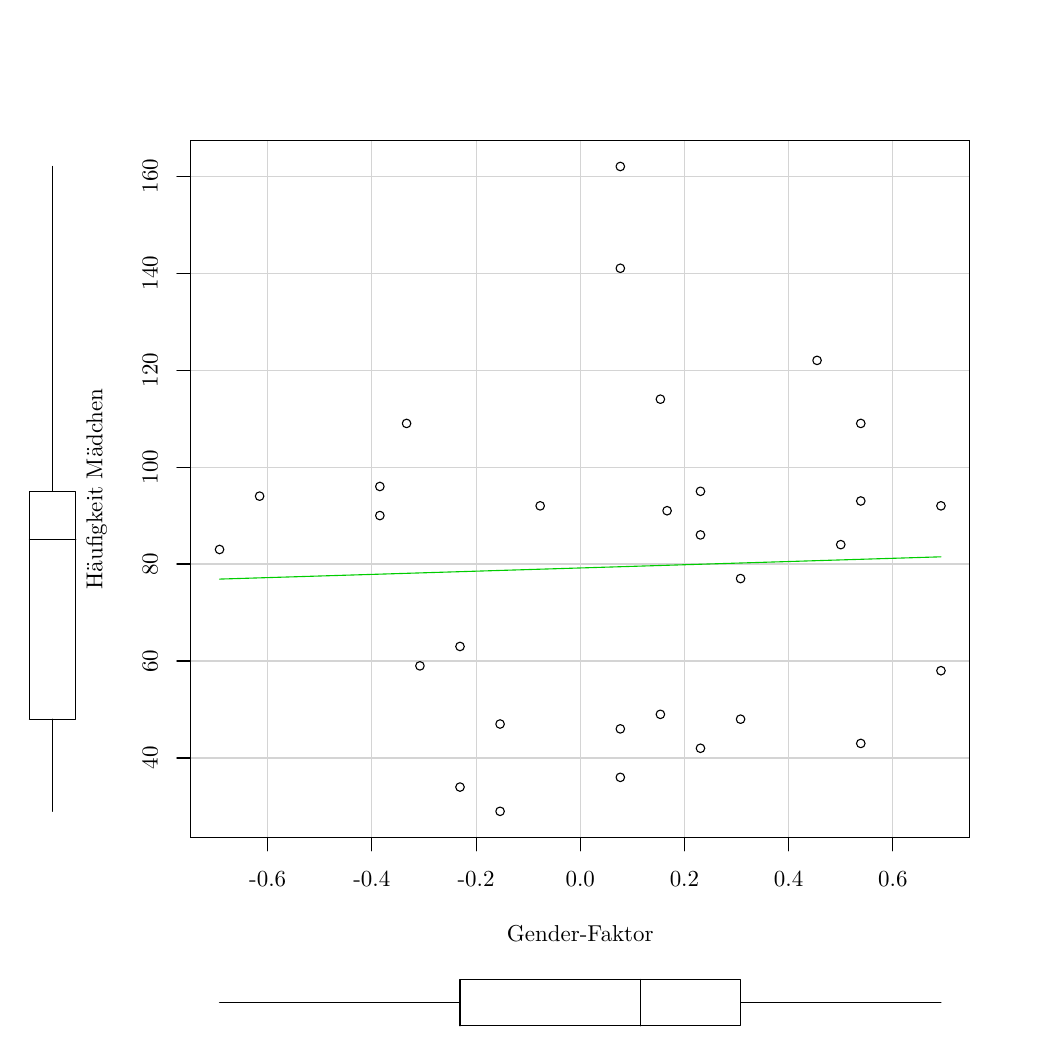
\begin{tikzpicture}[x=1pt,y=1pt]
\definecolor[named]{fillColor}{rgb}{1.00,1.00,1.00}
\path[use as bounding box,fill=fillColor,fill opacity=0.00] (0,0) rectangle (361.35,361.35);
\begin{scope}
\path[clip] (  0.00, 68.86) rectangle ( 18.07,320.51);
\definecolor[named]{drawColor}{rgb}{0.00,0.00,0.00}

\path[draw=drawColor,line width= 0.4pt,line join=round,line cap=round] (  0.67,111.47) --
	( 17.40,111.47) --
	( 17.40,193.81) --
	(  0.67,193.81) --
	(  0.67,111.47);

\path[draw=drawColor,line width= 0.4pt,line join=round,line cap=round] (  0.67,176.29) --
	( 17.40,176.29);

\path[draw=drawColor,line width= 0.4pt,line join=round,line cap=round] (  9.03, 78.18) --
	(  9.03,111.47);

\path[draw=drawColor,line width= 0.4pt,line join=round,line cap=round] (  9.03,193.81) --
	(  9.03,311.19);
\end{scope}
\begin{scope}
\path[clip] ( 58.90,  0.00) rectangle (340.43, 18.07);
\definecolor[named]{drawColor}{rgb}{0.00,0.00,0.00}

\path[draw=drawColor,line width= 0.4pt,line join=round,line cap=round] (156.22,  0.67) --
	(156.22, 17.40) --
	(257.60, 17.40) --
	(257.60,  0.67) --
	(156.22,  0.67);

\path[draw=drawColor,line width= 0.4pt,line join=round,line cap=round] (221.39,  0.67) --
	(221.39, 17.40);

\path[draw=drawColor,line width= 0.4pt,line join=round,line cap=round] ( 69.33,  9.03) --
	(156.22,  9.03);

\path[draw=drawColor,line width= 0.4pt,line join=round,line cap=round] (257.60,  9.03) --
	(330.01,  9.03);
\end{scope}
\begin{scope}
\path[clip] (  0.00,  0.00) rectangle (361.35,361.35);
\definecolor[named]{drawColor}{rgb}{0.00,0.00,0.00}

\path[draw=drawColor,line width= 0.4pt,line join=round,line cap=round] ( 86.71, 68.86) -- (312.63, 68.86);

\path[draw=drawColor,line width= 0.4pt,line join=round,line cap=round] ( 86.71, 68.86) -- ( 86.71, 63.88);

\path[draw=drawColor,line width= 0.4pt,line join=round,line cap=round] (124.36, 68.86) -- (124.36, 63.88);

\path[draw=drawColor,line width= 0.4pt,line join=round,line cap=round] (162.02, 68.86) -- (162.02, 63.88);

\path[draw=drawColor,line width= 0.4pt,line join=round,line cap=round] (199.67, 68.86) -- (199.67, 63.88);

\path[draw=drawColor,line width= 0.4pt,line join=round,line cap=round] (237.32, 68.86) -- (237.32, 63.88);

\path[draw=drawColor,line width= 0.4pt,line join=round,line cap=round] (274.98, 68.86) -- (274.98, 63.88);

\path[draw=drawColor,line width= 0.4pt,line join=round,line cap=round] (312.63, 68.86) -- (312.63, 63.88);

\node[text=drawColor,anchor=base,inner sep=0pt, outer sep=0pt, scale=  0.83] at ( 86.71, 50.94) {-0.6};

\node[text=drawColor,anchor=base,inner sep=0pt, outer sep=0pt, scale=  0.83] at (124.36, 50.94) {-0.4};

\node[text=drawColor,anchor=base,inner sep=0pt, outer sep=0pt, scale=  0.83] at (162.02, 50.94) {-0.2};

\node[text=drawColor,anchor=base,inner sep=0pt, outer sep=0pt, scale=  0.83] at (199.67, 50.94) {0.0};

\node[text=drawColor,anchor=base,inner sep=0pt, outer sep=0pt, scale=  0.83] at (237.32, 50.94) {0.2};

\node[text=drawColor,anchor=base,inner sep=0pt, outer sep=0pt, scale=  0.83] at (274.98, 50.94) {0.4};

\node[text=drawColor,anchor=base,inner sep=0pt, outer sep=0pt, scale=  0.83] at (312.63, 50.94) {0.6};

\path[draw=drawColor,line width= 0.4pt,line join=round,line cap=round] ( 58.90, 97.46) -- ( 58.90,307.69);

\path[draw=drawColor,line width= 0.4pt,line join=round,line cap=round] ( 58.90, 97.46) -- ( 53.92, 97.46);

\path[draw=drawColor,line width= 0.4pt,line join=round,line cap=round] ( 58.90,132.49) -- ( 53.92,132.49);

\path[draw=drawColor,line width= 0.4pt,line join=round,line cap=round] ( 58.90,167.53) -- ( 53.92,167.53);

\path[draw=drawColor,line width= 0.4pt,line join=round,line cap=round] ( 58.90,202.57) -- ( 53.92,202.57);

\path[draw=drawColor,line width= 0.4pt,line join=round,line cap=round] ( 58.90,237.61) -- ( 53.92,237.61);

\path[draw=drawColor,line width= 0.4pt,line join=round,line cap=round] ( 58.90,272.65) -- ( 53.92,272.65);

\path[draw=drawColor,line width= 0.4pt,line join=round,line cap=round] ( 58.90,307.69) -- ( 53.92,307.69);

\node[text=drawColor,rotate= 90.00,anchor=base,inner sep=0pt, outer sep=0pt, scale=  0.83] at ( 46.95, 97.46) {40};

\node[text=drawColor,rotate= 90.00,anchor=base,inner sep=0pt, outer sep=0pt, scale=  0.83] at ( 46.95,132.49) {60};

\node[text=drawColor,rotate= 90.00,anchor=base,inner sep=0pt, outer sep=0pt, scale=  0.83] at ( 46.95,167.53) {80};

\node[text=drawColor,rotate= 90.00,anchor=base,inner sep=0pt, outer sep=0pt, scale=  0.83] at ( 46.95,202.57) {100};

\node[text=drawColor,rotate= 90.00,anchor=base,inner sep=0pt, outer sep=0pt, scale=  0.83] at ( 46.95,237.61) {120};

\node[text=drawColor,rotate= 90.00,anchor=base,inner sep=0pt, outer sep=0pt, scale=  0.83] at ( 46.95,272.65) {140};

\node[text=drawColor,rotate= 90.00,anchor=base,inner sep=0pt, outer sep=0pt, scale=  0.83] at ( 46.95,307.69) {160};

\path[draw=drawColor,line width= 0.4pt,line join=round,line cap=round] ( 58.90, 68.86) --
	(340.43, 68.86) --
	(340.43,320.51) --
	( 58.90,320.51) --
	( 58.90, 68.86);
\end{scope}
\begin{scope}
\path[clip] ( 18.07, 18.07) rectangle (361.35,361.35);
\definecolor[named]{drawColor}{rgb}{0.00,0.00,0.00}

\node[text=drawColor,anchor=base,inner sep=0pt, outer sep=0pt, scale=  0.83] at (199.67, 31.02) {Gender-Faktor};

\node[text=drawColor,rotate= 90.00,anchor=base,inner sep=0pt, outer sep=0pt, scale=  0.83] at ( 27.03,194.69) {Häufigkeit Mädchen};
\end{scope}
\begin{scope}
\path[clip] ( 58.90, 68.86) rectangle (340.43,320.51);
\definecolor[named]{drawColor}{rgb}{0.83,0.83,0.83}

\path[draw=drawColor,line width= 0.4pt,line join=round,line cap=round] ( 86.71, 68.86) -- ( 86.71,320.51);

\path[draw=drawColor,line width= 0.4pt,line join=round,line cap=round] (124.36, 68.86) -- (124.36,320.51);

\path[draw=drawColor,line width= 0.4pt,line join=round,line cap=round] (162.02, 68.86) -- (162.02,320.51);

\path[draw=drawColor,line width= 0.4pt,line join=round,line cap=round] (199.67, 68.86) -- (199.67,320.51);

\path[draw=drawColor,line width= 0.4pt,line join=round,line cap=round] (237.32, 68.86) -- (237.32,320.51);

\path[draw=drawColor,line width= 0.4pt,line join=round,line cap=round] (274.98, 68.86) -- (274.98,320.51);

\path[draw=drawColor,line width= 0.4pt,line join=round,line cap=round] (312.63, 68.86) -- (312.63,320.51);

\path[draw=drawColor,line width= 0.4pt,line join=round,line cap=round] ( 58.90, 97.46) -- (340.43, 97.46);

\path[draw=drawColor,line width= 0.4pt,line join=round,line cap=round] ( 58.90,132.49) -- (340.43,132.49);

\path[draw=drawColor,line width= 0.4pt,line join=round,line cap=round] ( 58.90,167.53) -- (340.43,167.53);

\path[draw=drawColor,line width= 0.4pt,line join=round,line cap=round] ( 58.90,202.57) -- (340.43,202.57);

\path[draw=drawColor,line width= 0.4pt,line join=round,line cap=round] ( 58.90,237.61) -- (340.43,237.61);

\path[draw=drawColor,line width= 0.4pt,line join=round,line cap=round] ( 58.90,272.65) -- (340.43,272.65);

\path[draw=drawColor,line width= 0.4pt,line join=round,line cap=round] ( 58.90,307.69) -- (340.43,307.69);
\end{scope}
\begin{scope}
\path[clip] (  0.00,  0.00) rectangle (361.35,361.35);
\definecolor[named]{drawColor}{rgb}{0.00,0.00,0.00}

\path[draw=drawColor,line width= 0.4pt,line join=round,line cap=round] ( 58.90, 68.86) --
	(340.43, 68.86) --
	(340.43,320.51) --
	( 58.90,320.51) --
	( 58.90, 68.86);
\end{scope}
\begin{scope}
\path[clip] ( 58.90, 68.86) rectangle (340.43,320.51);
\definecolor[named]{drawColor}{rgb}{0.00,0.00,0.00}

\path[draw=drawColor,line width= 0.4pt,line join=round,line cap=round] (214.15,107.97) circle (  1.55);

\path[draw=drawColor,line width= 0.4pt,line join=round,line cap=round] (170.70, 78.18) circle (  1.55);

\path[draw=drawColor,line width= 0.4pt,line join=round,line cap=round] (170.70,109.72) circle (  1.55);

\path[draw=drawColor,line width= 0.4pt,line join=round,line cap=round] (228.63,227.10) circle (  1.55);

\path[draw=drawColor,line width= 0.4pt,line join=round,line cap=round] (228.63,113.22) circle (  1.55);

\path[draw=drawColor,line width= 0.4pt,line join=round,line cap=round] (257.60,111.47) circle (  1.55);

\path[draw=drawColor,line width= 0.4pt,line join=round,line cap=round] (293.80,174.54) circle (  1.55);

\path[draw=drawColor,line width= 0.4pt,line join=round,line cap=round] (136.91,218.34) circle (  1.55);

\path[draw=drawColor,line width= 0.4pt,line join=round,line cap=round] (214.15,311.19) circle (  1.55);

\path[draw=drawColor,line width= 0.4pt,line join=round,line cap=round] ( 83.81,192.06) circle (  1.55);

\path[draw=drawColor,line width= 0.4pt,line join=round,line cap=round] (214.15,274.40) circle (  1.55);

\path[draw=drawColor,line width= 0.4pt,line join=round,line cap=round] (141.74,130.74) circle (  1.55);

\path[draw=drawColor,line width= 0.4pt,line join=round,line cap=round] (257.60,162.28) circle (  1.55);

\path[draw=drawColor,line width= 0.4pt,line join=round,line cap=round] (301.04,218.34) circle (  1.55);

\path[draw=drawColor,line width= 0.4pt,line join=round,line cap=round] (231.05,186.80) circle (  1.55);

\path[draw=drawColor,line width= 0.4pt,line join=round,line cap=round] (156.22, 86.94) circle (  1.55);

\path[draw=drawColor,line width= 0.4pt,line join=round,line cap=round] (214.15, 90.45) circle (  1.55);

\path[draw=drawColor,line width= 0.4pt,line join=round,line cap=round] (185.19,188.56) circle (  1.55);

\path[draw=drawColor,line width= 0.4pt,line join=round,line cap=round] (243.11,100.96) circle (  1.55);

\path[draw=drawColor,line width= 0.4pt,line join=round,line cap=round] (127.26,195.56) circle (  1.55);

\path[draw=drawColor,line width= 0.4pt,line join=round,line cap=round] (330.01,188.56) circle (  1.55);

\path[draw=drawColor,line width= 0.4pt,line join=round,line cap=round] (127.26,185.05) circle (  1.55);

\path[draw=drawColor,line width= 0.4pt,line join=round,line cap=round] (301.04,102.71) circle (  1.55);

\path[draw=drawColor,line width= 0.4pt,line join=round,line cap=round] ( 69.33,172.79) circle (  1.55);

\path[draw=drawColor,line width= 0.4pt,line join=round,line cap=round] (243.11,193.81) circle (  1.55);

\path[draw=drawColor,line width= 0.4pt,line join=round,line cap=round] (301.04,190.31) circle (  1.55);

\path[draw=drawColor,line width= 0.4pt,line join=round,line cap=round] (243.11,178.05) circle (  1.55);

\path[draw=drawColor,line width= 0.4pt,line join=round,line cap=round] (330.01,128.99) circle (  1.55);

\path[draw=drawColor,line width= 0.4pt,line join=round,line cap=round] (285.24,241.12) circle (  1.55);

\path[draw=drawColor,line width= 0.4pt,line join=round,line cap=round] (156.22,137.75) circle (  1.55);
\definecolor[named]{drawColor}{rgb}{0.00,0.80,0.00}

\path[draw=drawColor,line width= 0.4pt,line join=round,line cap=round] ( 69.33,162.09) --
	(330.01,170.14);
\end{scope}
\end{tikzpicture}
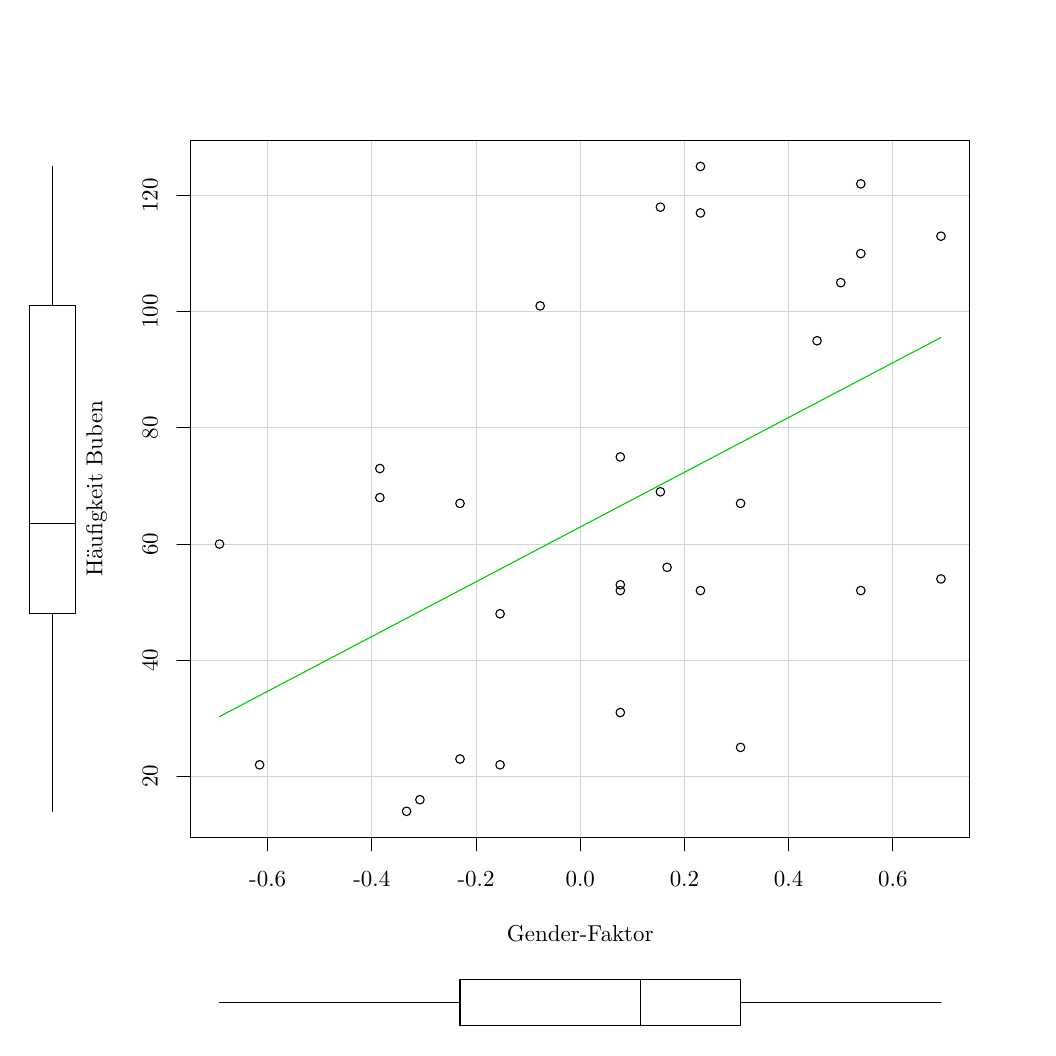
\begin{tikzpicture}[x=1pt,y=1pt]
\definecolor[named]{fillColor}{rgb}{1.00,1.00,1.00}
\path[use as bounding box,fill=fillColor,fill opacity=0.00] (0,0) rectangle (361.35,361.35);
\begin{scope}
\path[clip] (  0.00, 68.86) rectangle ( 18.07,320.51);
\definecolor[named]{drawColor}{rgb}{0.00,0.00,0.00}

\path[draw=drawColor,line width= 0.4pt,line join=round,line cap=round] (  0.67,149.56) --
	( 17.40,149.56) --
	( 17.40,260.81) --
	(  0.67,260.81) --
	(  0.67,149.56);

\path[draw=drawColor,line width= 0.4pt,line join=round,line cap=round] (  0.67,182.09) --
	( 17.40,182.09);

\path[draw=drawColor,line width= 0.4pt,line join=round,line cap=round] (  9.03, 78.18) --
	(  9.03,149.56);

\path[draw=drawColor,line width= 0.4pt,line join=round,line cap=round] (  9.03,260.81) --
	(  9.03,311.19);
\end{scope}
\begin{scope}
\path[clip] ( 58.90,  0.00) rectangle (340.43, 18.07);
\definecolor[named]{drawColor}{rgb}{0.00,0.00,0.00}

\path[draw=drawColor,line width= 0.4pt,line join=round,line cap=round] (156.22,  0.67) --
	(156.22, 17.40) --
	(257.60, 17.40) --
	(257.60,  0.67) --
	(156.22,  0.67);

\path[draw=drawColor,line width= 0.4pt,line join=round,line cap=round] (221.39,  0.67) --
	(221.39, 17.40);

\path[draw=drawColor,line width= 0.4pt,line join=round,line cap=round] ( 69.33,  9.03) --
	(156.22,  9.03);

\path[draw=drawColor,line width= 0.4pt,line join=round,line cap=round] (257.60,  9.03) --
	(330.01,  9.03);
\end{scope}
\begin{scope}
\path[clip] (  0.00,  0.00) rectangle (361.35,361.35);
\definecolor[named]{drawColor}{rgb}{0.00,0.00,0.00}

\path[draw=drawColor,line width= 0.4pt,line join=round,line cap=round] ( 86.71, 68.86) -- (312.63, 68.86);

\path[draw=drawColor,line width= 0.4pt,line join=round,line cap=round] ( 86.71, 68.86) -- ( 86.71, 63.88);

\path[draw=drawColor,line width= 0.4pt,line join=round,line cap=round] (124.36, 68.86) -- (124.36, 63.88);

\path[draw=drawColor,line width= 0.4pt,line join=round,line cap=round] (162.02, 68.86) -- (162.02, 63.88);

\path[draw=drawColor,line width= 0.4pt,line join=round,line cap=round] (199.67, 68.86) -- (199.67, 63.88);

\path[draw=drawColor,line width= 0.4pt,line join=round,line cap=round] (237.32, 68.86) -- (237.32, 63.88);

\path[draw=drawColor,line width= 0.4pt,line join=round,line cap=round] (274.98, 68.86) -- (274.98, 63.88);

\path[draw=drawColor,line width= 0.4pt,line join=round,line cap=round] (312.63, 68.86) -- (312.63, 63.88);

\node[text=drawColor,anchor=base,inner sep=0pt, outer sep=0pt, scale=  0.83] at ( 86.71, 50.94) {-0.6};

\node[text=drawColor,anchor=base,inner sep=0pt, outer sep=0pt, scale=  0.83] at (124.36, 50.94) {-0.4};

\node[text=drawColor,anchor=base,inner sep=0pt, outer sep=0pt, scale=  0.83] at (162.02, 50.94) {-0.2};

\node[text=drawColor,anchor=base,inner sep=0pt, outer sep=0pt, scale=  0.83] at (199.67, 50.94) {0.0};

\node[text=drawColor,anchor=base,inner sep=0pt, outer sep=0pt, scale=  0.83] at (237.32, 50.94) {0.2};

\node[text=drawColor,anchor=base,inner sep=0pt, outer sep=0pt, scale=  0.83] at (274.98, 50.94) {0.4};

\node[text=drawColor,anchor=base,inner sep=0pt, outer sep=0pt, scale=  0.83] at (312.63, 50.94) {0.6};

\path[draw=drawColor,line width= 0.4pt,line join=round,line cap=round] ( 58.90, 90.78) -- ( 58.90,300.70);

\path[draw=drawColor,line width= 0.4pt,line join=round,line cap=round] ( 58.90, 90.78) -- ( 53.92, 90.78);

\path[draw=drawColor,line width= 0.4pt,line join=round,line cap=round] ( 58.90,132.76) -- ( 53.92,132.76);

\path[draw=drawColor,line width= 0.4pt,line join=round,line cap=round] ( 58.90,174.75) -- ( 53.92,174.75);

\path[draw=drawColor,line width= 0.4pt,line join=round,line cap=round] ( 58.90,216.73) -- ( 53.92,216.73);

\path[draw=drawColor,line width= 0.4pt,line join=round,line cap=round] ( 58.90,258.71) -- ( 53.92,258.71);

\path[draw=drawColor,line width= 0.4pt,line join=round,line cap=round] ( 58.90,300.70) -- ( 53.92,300.70);

\node[text=drawColor,rotate= 90.00,anchor=base,inner sep=0pt, outer sep=0pt, scale=  0.83] at ( 46.95, 90.78) {20};

\node[text=drawColor,rotate= 90.00,anchor=base,inner sep=0pt, outer sep=0pt, scale=  0.83] at ( 46.95,132.76) {40};

\node[text=drawColor,rotate= 90.00,anchor=base,inner sep=0pt, outer sep=0pt, scale=  0.83] at ( 46.95,174.75) {60};

\node[text=drawColor,rotate= 90.00,anchor=base,inner sep=0pt, outer sep=0pt, scale=  0.83] at ( 46.95,216.73) {80};

\node[text=drawColor,rotate= 90.00,anchor=base,inner sep=0pt, outer sep=0pt, scale=  0.83] at ( 46.95,258.71) {100};

\node[text=drawColor,rotate= 90.00,anchor=base,inner sep=0pt, outer sep=0pt, scale=  0.83] at ( 46.95,300.70) {120};

\path[draw=drawColor,line width= 0.4pt,line join=round,line cap=round] ( 58.90, 68.86) --
	(340.43, 68.86) --
	(340.43,320.51) --
	( 58.90,320.51) --
	( 58.90, 68.86);
\end{scope}
\begin{scope}
\path[clip] ( 18.07, 18.07) rectangle (361.35,361.35);
\definecolor[named]{drawColor}{rgb}{0.00,0.00,0.00}

\node[text=drawColor,anchor=base,inner sep=0pt, outer sep=0pt, scale=  0.83] at (199.67, 31.02) {Gender-Faktor};

\node[text=drawColor,rotate= 90.00,anchor=base,inner sep=0pt, outer sep=0pt, scale=  0.83] at ( 27.03,194.69) {Häufigkeit Buben};
\end{scope}
\begin{scope}
\path[clip] ( 58.90, 68.86) rectangle (340.43,320.51);
\definecolor[named]{drawColor}{rgb}{0.83,0.83,0.83}

\path[draw=drawColor,line width= 0.4pt,line join=round,line cap=round] ( 86.71, 68.86) -- ( 86.71,320.51);

\path[draw=drawColor,line width= 0.4pt,line join=round,line cap=round] (124.36, 68.86) -- (124.36,320.51);

\path[draw=drawColor,line width= 0.4pt,line join=round,line cap=round] (162.02, 68.86) -- (162.02,320.51);

\path[draw=drawColor,line width= 0.4pt,line join=round,line cap=round] (199.67, 68.86) -- (199.67,320.51);

\path[draw=drawColor,line width= 0.4pt,line join=round,line cap=round] (237.32, 68.86) -- (237.32,320.51);

\path[draw=drawColor,line width= 0.4pt,line join=round,line cap=round] (274.98, 68.86) -- (274.98,320.51);

\path[draw=drawColor,line width= 0.4pt,line join=round,line cap=round] (312.63, 68.86) -- (312.63,320.51);

\path[draw=drawColor,line width= 0.4pt,line join=round,line cap=round] ( 58.90, 90.78) -- (340.43, 90.78);

\path[draw=drawColor,line width= 0.4pt,line join=round,line cap=round] ( 58.90,132.76) -- (340.43,132.76);

\path[draw=drawColor,line width= 0.4pt,line join=round,line cap=round] ( 58.90,174.75) -- (340.43,174.75);

\path[draw=drawColor,line width= 0.4pt,line join=round,line cap=round] ( 58.90,216.73) -- (340.43,216.73);

\path[draw=drawColor,line width= 0.4pt,line join=round,line cap=round] ( 58.90,258.71) -- (340.43,258.71);

\path[draw=drawColor,line width= 0.4pt,line join=round,line cap=round] ( 58.90,300.70) -- (340.43,300.70);
\end{scope}
\begin{scope}
\path[clip] (  0.00,  0.00) rectangle (361.35,361.35);
\definecolor[named]{drawColor}{rgb}{0.00,0.00,0.00}

\path[draw=drawColor,line width= 0.4pt,line join=round,line cap=round] ( 58.90, 68.86) --
	(340.43, 68.86) --
	(340.43,320.51) --
	( 58.90,320.51) --
	( 58.90, 68.86);
\end{scope}
\begin{scope}
\path[clip] ( 58.90, 68.86) rectangle (340.43,320.51);
\definecolor[named]{drawColor}{rgb}{0.00,0.00,0.00}

\path[draw=drawColor,line width= 0.4pt,line join=round,line cap=round] (214.15,157.95) circle (  1.55);

\path[draw=drawColor,line width= 0.4pt,line join=round,line cap=round] (170.70, 94.98) circle (  1.55);

\path[draw=drawColor,line width= 0.4pt,line join=round,line cap=round] (170.70,149.56) circle (  1.55);

\path[draw=drawColor,line width= 0.4pt,line join=round,line cap=round] (228.63,296.50) circle (  1.55);

\path[draw=drawColor,line width= 0.4pt,line join=round,line cap=round] (228.63,193.64) circle (  1.55);

\path[draw=drawColor,line width= 0.4pt,line join=round,line cap=round] (257.60,189.44) circle (  1.55);

\path[draw=drawColor,line width= 0.4pt,line join=round,line cap=round] (293.80,269.21) circle (  1.55);

\path[draw=drawColor,line width= 0.4pt,line join=round,line cap=round] (136.91, 78.18) circle (  1.55);

\path[draw=drawColor,line width= 0.4pt,line join=round,line cap=round] (214.15,160.05) circle (  1.55);

\path[draw=drawColor,line width= 0.4pt,line join=round,line cap=round] ( 83.81, 94.98) circle (  1.55);

\path[draw=drawColor,line width= 0.4pt,line join=round,line cap=round] (214.15,206.23) circle (  1.55);

\path[draw=drawColor,line width= 0.4pt,line join=round,line cap=round] (141.74, 82.38) circle (  1.55);

\path[draw=drawColor,line width= 0.4pt,line join=round,line cap=round] (257.60,101.27) circle (  1.55);

\path[draw=drawColor,line width= 0.4pt,line join=round,line cap=round] (301.04,157.95) circle (  1.55);

\path[draw=drawColor,line width= 0.4pt,line join=round,line cap=round] (231.05,166.35) circle (  1.55);

\path[draw=drawColor,line width= 0.4pt,line join=round,line cap=round] (156.22, 97.08) circle (  1.55);

\path[draw=drawColor,line width= 0.4pt,line join=round,line cap=round] (214.15,113.87) circle (  1.55);

\path[draw=drawColor,line width= 0.4pt,line join=round,line cap=round] (185.19,260.81) circle (  1.55);

\path[draw=drawColor,line width= 0.4pt,line join=round,line cap=round] (243.11,157.95) circle (  1.55);

\path[draw=drawColor,line width= 0.4pt,line join=round,line cap=round] (127.26,191.54) circle (  1.55);

\path[draw=drawColor,line width= 0.4pt,line join=round,line cap=round] (330.01,286.00) circle (  1.55);

\path[draw=drawColor,line width= 0.4pt,line join=round,line cap=round] (127.26,202.04) circle (  1.55);

\path[draw=drawColor,line width= 0.4pt,line join=round,line cap=round] (301.04,279.71) circle (  1.55);

\path[draw=drawColor,line width= 0.4pt,line join=round,line cap=round] ( 69.33,174.75) circle (  1.55);

\path[draw=drawColor,line width= 0.4pt,line join=round,line cap=round] (243.11,311.19) circle (  1.55);

\path[draw=drawColor,line width= 0.4pt,line join=round,line cap=round] (301.04,304.90) circle (  1.55);

\path[draw=drawColor,line width= 0.4pt,line join=round,line cap=round] (243.11,294.40) circle (  1.55);

\path[draw=drawColor,line width= 0.4pt,line join=round,line cap=round] (330.01,162.15) circle (  1.55);

\path[draw=drawColor,line width= 0.4pt,line join=round,line cap=round] (285.24,248.22) circle (  1.55);

\path[draw=drawColor,line width= 0.4pt,line join=round,line cap=round] (156.22,189.44) circle (  1.55);
\definecolor[named]{drawColor}{rgb}{0.00,0.80,0.00}

\path[draw=drawColor,line width= 0.4pt,line join=round,line cap=round] ( 69.33,112.42) --
	(330.01,249.40);
\end{scope}
\end{tikzpicture}
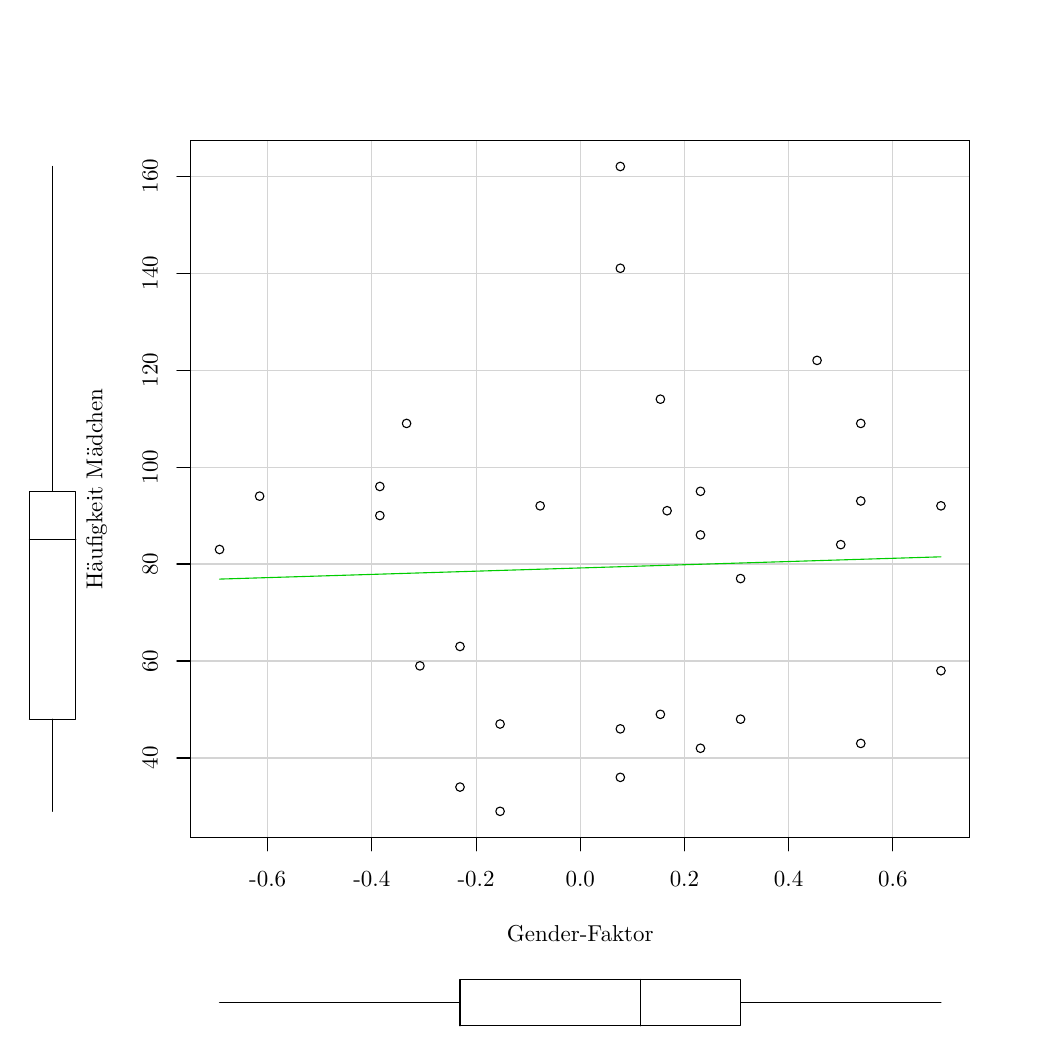
\begin{tikzpicture}[x=1pt,y=1pt]
\definecolor[named]{fillColor}{rgb}{1.00,1.00,1.00}
\path[use as bounding box,fill=fillColor,fill opacity=0.00] (0,0) rectangle (361.35,361.35);
\begin{scope}
\path[clip] (  0.00, 68.86) rectangle ( 18.07,320.51);
\definecolor[named]{drawColor}{rgb}{0.00,0.00,0.00}

\path[draw=drawColor,line width= 0.4pt,line join=round,line cap=round] (  0.67,111.47) --
	( 17.40,111.47) --
	( 17.40,193.81) --
	(  0.67,193.81) --
	(  0.67,111.47);

\path[draw=drawColor,line width= 0.4pt,line join=round,line cap=round] (  0.67,176.29) --
	( 17.40,176.29);

\path[draw=drawColor,line width= 0.4pt,line join=round,line cap=round] (  9.03, 78.18) --
	(  9.03,111.47);

\path[draw=drawColor,line width= 0.4pt,line join=round,line cap=round] (  9.03,193.81) --
	(  9.03,311.19);
\end{scope}
\begin{scope}
\path[clip] ( 58.90,  0.00) rectangle (340.43, 18.07);
\definecolor[named]{drawColor}{rgb}{0.00,0.00,0.00}

\path[draw=drawColor,line width= 0.4pt,line join=round,line cap=round] (156.22,  0.67) --
	(156.22, 17.40) --
	(257.60, 17.40) --
	(257.60,  0.67) --
	(156.22,  0.67);

\path[draw=drawColor,line width= 0.4pt,line join=round,line cap=round] (221.39,  0.67) --
	(221.39, 17.40);

\path[draw=drawColor,line width= 0.4pt,line join=round,line cap=round] ( 69.33,  9.03) --
	(156.22,  9.03);

\path[draw=drawColor,line width= 0.4pt,line join=round,line cap=round] (257.60,  9.03) --
	(330.01,  9.03);
\end{scope}
\begin{scope}
\path[clip] (  0.00,  0.00) rectangle (361.35,361.35);
\definecolor[named]{drawColor}{rgb}{0.00,0.00,0.00}

\path[draw=drawColor,line width= 0.4pt,line join=round,line cap=round] ( 86.71, 68.86) -- (312.63, 68.86);

\path[draw=drawColor,line width= 0.4pt,line join=round,line cap=round] ( 86.71, 68.86) -- ( 86.71, 63.88);

\path[draw=drawColor,line width= 0.4pt,line join=round,line cap=round] (124.36, 68.86) -- (124.36, 63.88);

\path[draw=drawColor,line width= 0.4pt,line join=round,line cap=round] (162.02, 68.86) -- (162.02, 63.88);

\path[draw=drawColor,line width= 0.4pt,line join=round,line cap=round] (199.67, 68.86) -- (199.67, 63.88);

\path[draw=drawColor,line width= 0.4pt,line join=round,line cap=round] (237.32, 68.86) -- (237.32, 63.88);

\path[draw=drawColor,line width= 0.4pt,line join=round,line cap=round] (274.98, 68.86) -- (274.98, 63.88);

\path[draw=drawColor,line width= 0.4pt,line join=round,line cap=round] (312.63, 68.86) -- (312.63, 63.88);

\node[text=drawColor,anchor=base,inner sep=0pt, outer sep=0pt, scale=  0.83] at ( 86.71, 50.94) {-0.6};

\node[text=drawColor,anchor=base,inner sep=0pt, outer sep=0pt, scale=  0.83] at (124.36, 50.94) {-0.4};

\node[text=drawColor,anchor=base,inner sep=0pt, outer sep=0pt, scale=  0.83] at (162.02, 50.94) {-0.2};

\node[text=drawColor,anchor=base,inner sep=0pt, outer sep=0pt, scale=  0.83] at (199.67, 50.94) {0.0};

\node[text=drawColor,anchor=base,inner sep=0pt, outer sep=0pt, scale=  0.83] at (237.32, 50.94) {0.2};

\node[text=drawColor,anchor=base,inner sep=0pt, outer sep=0pt, scale=  0.83] at (274.98, 50.94) {0.4};

\node[text=drawColor,anchor=base,inner sep=0pt, outer sep=0pt, scale=  0.83] at (312.63, 50.94) {0.6};

\path[draw=drawColor,line width= 0.4pt,line join=round,line cap=round] ( 58.90, 97.46) -- ( 58.90,307.69);

\path[draw=drawColor,line width= 0.4pt,line join=round,line cap=round] ( 58.90, 97.46) -- ( 53.92, 97.46);

\path[draw=drawColor,line width= 0.4pt,line join=round,line cap=round] ( 58.90,132.49) -- ( 53.92,132.49);

\path[draw=drawColor,line width= 0.4pt,line join=round,line cap=round] ( 58.90,167.53) -- ( 53.92,167.53);

\path[draw=drawColor,line width= 0.4pt,line join=round,line cap=round] ( 58.90,202.57) -- ( 53.92,202.57);

\path[draw=drawColor,line width= 0.4pt,line join=round,line cap=round] ( 58.90,237.61) -- ( 53.92,237.61);

\path[draw=drawColor,line width= 0.4pt,line join=round,line cap=round] ( 58.90,272.65) -- ( 53.92,272.65);

\path[draw=drawColor,line width= 0.4pt,line join=round,line cap=round] ( 58.90,307.69) -- ( 53.92,307.69);

\node[text=drawColor,rotate= 90.00,anchor=base,inner sep=0pt, outer sep=0pt, scale=  0.83] at ( 46.95, 97.46) {40};

\node[text=drawColor,rotate= 90.00,anchor=base,inner sep=0pt, outer sep=0pt, scale=  0.83] at ( 46.95,132.49) {60};

\node[text=drawColor,rotate= 90.00,anchor=base,inner sep=0pt, outer sep=0pt, scale=  0.83] at ( 46.95,167.53) {80};

\node[text=drawColor,rotate= 90.00,anchor=base,inner sep=0pt, outer sep=0pt, scale=  0.83] at ( 46.95,202.57) {100};

\node[text=drawColor,rotate= 90.00,anchor=base,inner sep=0pt, outer sep=0pt, scale=  0.83] at ( 46.95,237.61) {120};

\node[text=drawColor,rotate= 90.00,anchor=base,inner sep=0pt, outer sep=0pt, scale=  0.83] at ( 46.95,272.65) {140};

\node[text=drawColor,rotate= 90.00,anchor=base,inner sep=0pt, outer sep=0pt, scale=  0.83] at ( 46.95,307.69) {160};

\path[draw=drawColor,line width= 0.4pt,line join=round,line cap=round] ( 58.90, 68.86) --
	(340.43, 68.86) --
	(340.43,320.51) --
	( 58.90,320.51) --
	( 58.90, 68.86);
\end{scope}
\begin{scope}
\path[clip] ( 18.07, 18.07) rectangle (361.35,361.35);
\definecolor[named]{drawColor}{rgb}{0.00,0.00,0.00}

\node[text=drawColor,anchor=base,inner sep=0pt, outer sep=0pt, scale=  0.83] at (199.67, 31.02) {Gender-Faktor};

\node[text=drawColor,rotate= 90.00,anchor=base,inner sep=0pt, outer sep=0pt, scale=  0.83] at ( 27.03,194.69) {Häufigkeit Mädchen};
\end{scope}
\begin{scope}
\path[clip] ( 58.90, 68.86) rectangle (340.43,320.51);
\definecolor[named]{drawColor}{rgb}{0.83,0.83,0.83}

\path[draw=drawColor,line width= 0.4pt,line join=round,line cap=round] ( 86.71, 68.86) -- ( 86.71,320.51);

\path[draw=drawColor,line width= 0.4pt,line join=round,line cap=round] (124.36, 68.86) -- (124.36,320.51);

\path[draw=drawColor,line width= 0.4pt,line join=round,line cap=round] (162.02, 68.86) -- (162.02,320.51);

\path[draw=drawColor,line width= 0.4pt,line join=round,line cap=round] (199.67, 68.86) -- (199.67,320.51);

\path[draw=drawColor,line width= 0.4pt,line join=round,line cap=round] (237.32, 68.86) -- (237.32,320.51);

\path[draw=drawColor,line width= 0.4pt,line join=round,line cap=round] (274.98, 68.86) -- (274.98,320.51);

\path[draw=drawColor,line width= 0.4pt,line join=round,line cap=round] (312.63, 68.86) -- (312.63,320.51);

\path[draw=drawColor,line width= 0.4pt,line join=round,line cap=round] ( 58.90, 97.46) -- (340.43, 97.46);

\path[draw=drawColor,line width= 0.4pt,line join=round,line cap=round] ( 58.90,132.49) -- (340.43,132.49);

\path[draw=drawColor,line width= 0.4pt,line join=round,line cap=round] ( 58.90,167.53) -- (340.43,167.53);

\path[draw=drawColor,line width= 0.4pt,line join=round,line cap=round] ( 58.90,202.57) -- (340.43,202.57);

\path[draw=drawColor,line width= 0.4pt,line join=round,line cap=round] ( 58.90,237.61) -- (340.43,237.61);

\path[draw=drawColor,line width= 0.4pt,line join=round,line cap=round] ( 58.90,272.65) -- (340.43,272.65);

\path[draw=drawColor,line width= 0.4pt,line join=round,line cap=round] ( 58.90,307.69) -- (340.43,307.69);
\end{scope}
\begin{scope}
\path[clip] (  0.00,  0.00) rectangle (361.35,361.35);
\definecolor[named]{drawColor}{rgb}{0.00,0.00,0.00}

\path[draw=drawColor,line width= 0.4pt,line join=round,line cap=round] ( 58.90, 68.86) --
	(340.43, 68.86) --
	(340.43,320.51) --
	( 58.90,320.51) --
	( 58.90, 68.86);
\end{scope}
\begin{scope}
\path[clip] ( 58.90, 68.86) rectangle (340.43,320.51);
\definecolor[named]{drawColor}{rgb}{0.00,0.00,0.00}

\path[draw=drawColor,line width= 0.4pt,line join=round,line cap=round] (214.15,107.97) circle (  1.55);

\path[draw=drawColor,line width= 0.4pt,line join=round,line cap=round] (170.70, 78.18) circle (  1.55);

\path[draw=drawColor,line width= 0.4pt,line join=round,line cap=round] (170.70,109.72) circle (  1.55);

\path[draw=drawColor,line width= 0.4pt,line join=round,line cap=round] (228.63,227.10) circle (  1.55);

\path[draw=drawColor,line width= 0.4pt,line join=round,line cap=round] (228.63,113.22) circle (  1.55);

\path[draw=drawColor,line width= 0.4pt,line join=round,line cap=round] (257.60,111.47) circle (  1.55);

\path[draw=drawColor,line width= 0.4pt,line join=round,line cap=round] (293.80,174.54) circle (  1.55);

\path[draw=drawColor,line width= 0.4pt,line join=round,line cap=round] (136.91,218.34) circle (  1.55);

\path[draw=drawColor,line width= 0.4pt,line join=round,line cap=round] (214.15,311.19) circle (  1.55);

\path[draw=drawColor,line width= 0.4pt,line join=round,line cap=round] ( 83.81,192.06) circle (  1.55);

\path[draw=drawColor,line width= 0.4pt,line join=round,line cap=round] (214.15,274.40) circle (  1.55);

\path[draw=drawColor,line width= 0.4pt,line join=round,line cap=round] (141.74,130.74) circle (  1.55);

\path[draw=drawColor,line width= 0.4pt,line join=round,line cap=round] (257.60,162.28) circle (  1.55);

\path[draw=drawColor,line width= 0.4pt,line join=round,line cap=round] (301.04,218.34) circle (  1.55);

\path[draw=drawColor,line width= 0.4pt,line join=round,line cap=round] (231.05,186.80) circle (  1.55);

\path[draw=drawColor,line width= 0.4pt,line join=round,line cap=round] (156.22, 86.94) circle (  1.55);

\path[draw=drawColor,line width= 0.4pt,line join=round,line cap=round] (214.15, 90.45) circle (  1.55);

\path[draw=drawColor,line width= 0.4pt,line join=round,line cap=round] (185.19,188.56) circle (  1.55);

\path[draw=drawColor,line width= 0.4pt,line join=round,line cap=round] (243.11,100.96) circle (  1.55);

\path[draw=drawColor,line width= 0.4pt,line join=round,line cap=round] (127.26,195.56) circle (  1.55);

\path[draw=drawColor,line width= 0.4pt,line join=round,line cap=round] (330.01,188.56) circle (  1.55);

\path[draw=drawColor,line width= 0.4pt,line join=round,line cap=round] (127.26,185.05) circle (  1.55);

\path[draw=drawColor,line width= 0.4pt,line join=round,line cap=round] (301.04,102.71) circle (  1.55);

\path[draw=drawColor,line width= 0.4pt,line join=round,line cap=round] ( 69.33,172.79) circle (  1.55);

\path[draw=drawColor,line width= 0.4pt,line join=round,line cap=round] (243.11,193.81) circle (  1.55);

\path[draw=drawColor,line width= 0.4pt,line join=round,line cap=round] (301.04,190.31) circle (  1.55);

\path[draw=drawColor,line width= 0.4pt,line join=round,line cap=round] (243.11,178.05) circle (  1.55);

\path[draw=drawColor,line width= 0.4pt,line join=round,line cap=round] (330.01,128.99) circle (  1.55);

\path[draw=drawColor,line width= 0.4pt,line join=round,line cap=round] (285.24,241.12) circle (  1.55);

\path[draw=drawColor,line width= 0.4pt,line join=round,line cap=round] (156.22,137.75) circle (  1.55);
\definecolor[named]{drawColor}{rgb}{0.00,0.80,0.00}

\path[draw=drawColor,line width= 0.4pt,line join=round,line cap=round] ( 69.33,162.09) --
	(330.01,170.14);
\end{scope}
\end{tikzpicture}
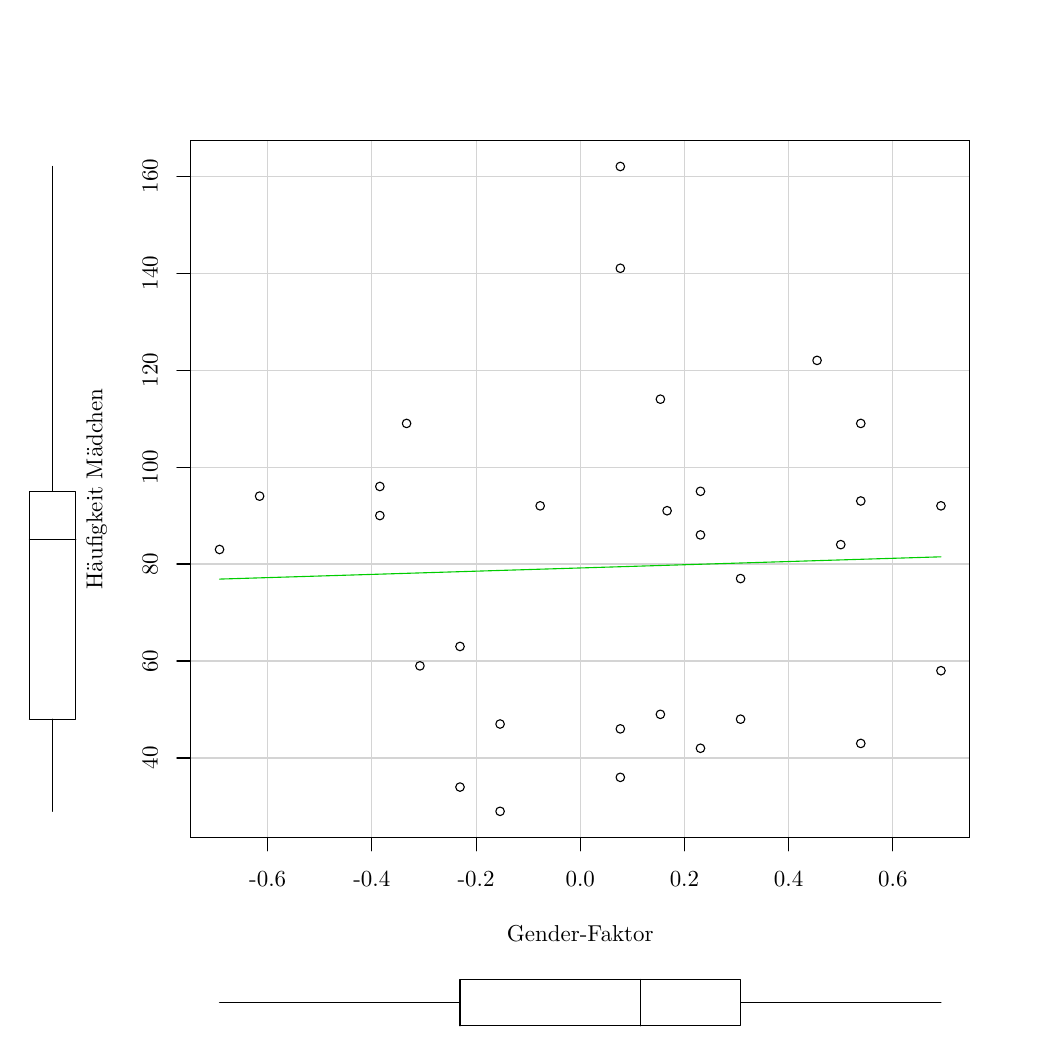
\begin{tikzpicture}[x=1pt,y=1pt]
\definecolor[named]{fillColor}{rgb}{1.00,1.00,1.00}
\path[use as bounding box,fill=fillColor,fill opacity=0.00] (0,0) rectangle (361.35,361.35);
\begin{scope}
\path[clip] (  0.00, 68.86) rectangle ( 18.07,320.51);
\definecolor[named]{drawColor}{rgb}{0.00,0.00,0.00}

\path[draw=drawColor,line width= 0.4pt,line join=round,line cap=round] (  0.67,111.47) --
	( 17.40,111.47) --
	( 17.40,193.81) --
	(  0.67,193.81) --
	(  0.67,111.47);

\path[draw=drawColor,line width= 0.4pt,line join=round,line cap=round] (  0.67,176.29) --
	( 17.40,176.29);

\path[draw=drawColor,line width= 0.4pt,line join=round,line cap=round] (  9.03, 78.18) --
	(  9.03,111.47);

\path[draw=drawColor,line width= 0.4pt,line join=round,line cap=round] (  9.03,193.81) --
	(  9.03,311.19);
\end{scope}
\begin{scope}
\path[clip] ( 58.90,  0.00) rectangle (340.43, 18.07);
\definecolor[named]{drawColor}{rgb}{0.00,0.00,0.00}

\path[draw=drawColor,line width= 0.4pt,line join=round,line cap=round] (156.22,  0.67) --
	(156.22, 17.40) --
	(257.60, 17.40) --
	(257.60,  0.67) --
	(156.22,  0.67);

\path[draw=drawColor,line width= 0.4pt,line join=round,line cap=round] (221.39,  0.67) --
	(221.39, 17.40);

\path[draw=drawColor,line width= 0.4pt,line join=round,line cap=round] ( 69.33,  9.03) --
	(156.22,  9.03);

\path[draw=drawColor,line width= 0.4pt,line join=round,line cap=round] (257.60,  9.03) --
	(330.01,  9.03);
\end{scope}
\begin{scope}
\path[clip] (  0.00,  0.00) rectangle (361.35,361.35);
\definecolor[named]{drawColor}{rgb}{0.00,0.00,0.00}

\path[draw=drawColor,line width= 0.4pt,line join=round,line cap=round] ( 86.71, 68.86) -- (312.63, 68.86);

\path[draw=drawColor,line width= 0.4pt,line join=round,line cap=round] ( 86.71, 68.86) -- ( 86.71, 63.88);

\path[draw=drawColor,line width= 0.4pt,line join=round,line cap=round] (124.36, 68.86) -- (124.36, 63.88);

\path[draw=drawColor,line width= 0.4pt,line join=round,line cap=round] (162.02, 68.86) -- (162.02, 63.88);

\path[draw=drawColor,line width= 0.4pt,line join=round,line cap=round] (199.67, 68.86) -- (199.67, 63.88);

\path[draw=drawColor,line width= 0.4pt,line join=round,line cap=round] (237.32, 68.86) -- (237.32, 63.88);

\path[draw=drawColor,line width= 0.4pt,line join=round,line cap=round] (274.98, 68.86) -- (274.98, 63.88);

\path[draw=drawColor,line width= 0.4pt,line join=round,line cap=round] (312.63, 68.86) -- (312.63, 63.88);

\node[text=drawColor,anchor=base,inner sep=0pt, outer sep=0pt, scale=  0.83] at ( 86.71, 50.94) {-0.6};

\node[text=drawColor,anchor=base,inner sep=0pt, outer sep=0pt, scale=  0.83] at (124.36, 50.94) {-0.4};

\node[text=drawColor,anchor=base,inner sep=0pt, outer sep=0pt, scale=  0.83] at (162.02, 50.94) {-0.2};

\node[text=drawColor,anchor=base,inner sep=0pt, outer sep=0pt, scale=  0.83] at (199.67, 50.94) {0.0};

\node[text=drawColor,anchor=base,inner sep=0pt, outer sep=0pt, scale=  0.83] at (237.32, 50.94) {0.2};

\node[text=drawColor,anchor=base,inner sep=0pt, outer sep=0pt, scale=  0.83] at (274.98, 50.94) {0.4};

\node[text=drawColor,anchor=base,inner sep=0pt, outer sep=0pt, scale=  0.83] at (312.63, 50.94) {0.6};

\path[draw=drawColor,line width= 0.4pt,line join=round,line cap=round] ( 58.90, 97.46) -- ( 58.90,307.69);

\path[draw=drawColor,line width= 0.4pt,line join=round,line cap=round] ( 58.90, 97.46) -- ( 53.92, 97.46);

\path[draw=drawColor,line width= 0.4pt,line join=round,line cap=round] ( 58.90,132.49) -- ( 53.92,132.49);

\path[draw=drawColor,line width= 0.4pt,line join=round,line cap=round] ( 58.90,167.53) -- ( 53.92,167.53);

\path[draw=drawColor,line width= 0.4pt,line join=round,line cap=round] ( 58.90,202.57) -- ( 53.92,202.57);

\path[draw=drawColor,line width= 0.4pt,line join=round,line cap=round] ( 58.90,237.61) -- ( 53.92,237.61);

\path[draw=drawColor,line width= 0.4pt,line join=round,line cap=round] ( 58.90,272.65) -- ( 53.92,272.65);

\path[draw=drawColor,line width= 0.4pt,line join=round,line cap=round] ( 58.90,307.69) -- ( 53.92,307.69);

\node[text=drawColor,rotate= 90.00,anchor=base,inner sep=0pt, outer sep=0pt, scale=  0.83] at ( 46.95, 97.46) {40};

\node[text=drawColor,rotate= 90.00,anchor=base,inner sep=0pt, outer sep=0pt, scale=  0.83] at ( 46.95,132.49) {60};

\node[text=drawColor,rotate= 90.00,anchor=base,inner sep=0pt, outer sep=0pt, scale=  0.83] at ( 46.95,167.53) {80};

\node[text=drawColor,rotate= 90.00,anchor=base,inner sep=0pt, outer sep=0pt, scale=  0.83] at ( 46.95,202.57) {100};

\node[text=drawColor,rotate= 90.00,anchor=base,inner sep=0pt, outer sep=0pt, scale=  0.83] at ( 46.95,237.61) {120};

\node[text=drawColor,rotate= 90.00,anchor=base,inner sep=0pt, outer sep=0pt, scale=  0.83] at ( 46.95,272.65) {140};

\node[text=drawColor,rotate= 90.00,anchor=base,inner sep=0pt, outer sep=0pt, scale=  0.83] at ( 46.95,307.69) {160};

\path[draw=drawColor,line width= 0.4pt,line join=round,line cap=round] ( 58.90, 68.86) --
	(340.43, 68.86) --
	(340.43,320.51) --
	( 58.90,320.51) --
	( 58.90, 68.86);
\end{scope}
\begin{scope}
\path[clip] ( 18.07, 18.07) rectangle (361.35,361.35);
\definecolor[named]{drawColor}{rgb}{0.00,0.00,0.00}

\node[text=drawColor,anchor=base,inner sep=0pt, outer sep=0pt, scale=  0.83] at (199.67, 31.02) {Gender-Faktor};

\node[text=drawColor,rotate= 90.00,anchor=base,inner sep=0pt, outer sep=0pt, scale=  0.83] at ( 27.03,194.69) {Häufigkeit Mädchen};
\end{scope}
\begin{scope}
\path[clip] ( 58.90, 68.86) rectangle (340.43,320.51);
\definecolor[named]{drawColor}{rgb}{0.83,0.83,0.83}

\path[draw=drawColor,line width= 0.4pt,line join=round,line cap=round] ( 86.71, 68.86) -- ( 86.71,320.51);

\path[draw=drawColor,line width= 0.4pt,line join=round,line cap=round] (124.36, 68.86) -- (124.36,320.51);

\path[draw=drawColor,line width= 0.4pt,line join=round,line cap=round] (162.02, 68.86) -- (162.02,320.51);

\path[draw=drawColor,line width= 0.4pt,line join=round,line cap=round] (199.67, 68.86) -- (199.67,320.51);

\path[draw=drawColor,line width= 0.4pt,line join=round,line cap=round] (237.32, 68.86) -- (237.32,320.51);

\path[draw=drawColor,line width= 0.4pt,line join=round,line cap=round] (274.98, 68.86) -- (274.98,320.51);

\path[draw=drawColor,line width= 0.4pt,line join=round,line cap=round] (312.63, 68.86) -- (312.63,320.51);

\path[draw=drawColor,line width= 0.4pt,line join=round,line cap=round] ( 58.90, 97.46) -- (340.43, 97.46);

\path[draw=drawColor,line width= 0.4pt,line join=round,line cap=round] ( 58.90,132.49) -- (340.43,132.49);

\path[draw=drawColor,line width= 0.4pt,line join=round,line cap=round] ( 58.90,167.53) -- (340.43,167.53);

\path[draw=drawColor,line width= 0.4pt,line join=round,line cap=round] ( 58.90,202.57) -- (340.43,202.57);

\path[draw=drawColor,line width= 0.4pt,line join=round,line cap=round] ( 58.90,237.61) -- (340.43,237.61);

\path[draw=drawColor,line width= 0.4pt,line join=round,line cap=round] ( 58.90,272.65) -- (340.43,272.65);

\path[draw=drawColor,line width= 0.4pt,line join=round,line cap=round] ( 58.90,307.69) -- (340.43,307.69);
\end{scope}
\begin{scope}
\path[clip] (  0.00,  0.00) rectangle (361.35,361.35);
\definecolor[named]{drawColor}{rgb}{0.00,0.00,0.00}

\path[draw=drawColor,line width= 0.4pt,line join=round,line cap=round] ( 58.90, 68.86) --
	(340.43, 68.86) --
	(340.43,320.51) --
	( 58.90,320.51) --
	( 58.90, 68.86);
\end{scope}
\begin{scope}
\path[clip] ( 58.90, 68.86) rectangle (340.43,320.51);
\definecolor[named]{drawColor}{rgb}{0.00,0.00,0.00}

\path[draw=drawColor,line width= 0.4pt,line join=round,line cap=round] (214.15,107.97) circle (  1.55);

\path[draw=drawColor,line width= 0.4pt,line join=round,line cap=round] (170.70, 78.18) circle (  1.55);

\path[draw=drawColor,line width= 0.4pt,line join=round,line cap=round] (170.70,109.72) circle (  1.55);

\path[draw=drawColor,line width= 0.4pt,line join=round,line cap=round] (228.63,227.10) circle (  1.55);

\path[draw=drawColor,line width= 0.4pt,line join=round,line cap=round] (228.63,113.22) circle (  1.55);

\path[draw=drawColor,line width= 0.4pt,line join=round,line cap=round] (257.60,111.47) circle (  1.55);

\path[draw=drawColor,line width= 0.4pt,line join=round,line cap=round] (293.80,174.54) circle (  1.55);

\path[draw=drawColor,line width= 0.4pt,line join=round,line cap=round] (136.91,218.34) circle (  1.55);

\path[draw=drawColor,line width= 0.4pt,line join=round,line cap=round] (214.15,311.19) circle (  1.55);

\path[draw=drawColor,line width= 0.4pt,line join=round,line cap=round] ( 83.81,192.06) circle (  1.55);

\path[draw=drawColor,line width= 0.4pt,line join=round,line cap=round] (214.15,274.40) circle (  1.55);

\path[draw=drawColor,line width= 0.4pt,line join=round,line cap=round] (141.74,130.74) circle (  1.55);

\path[draw=drawColor,line width= 0.4pt,line join=round,line cap=round] (257.60,162.28) circle (  1.55);

\path[draw=drawColor,line width= 0.4pt,line join=round,line cap=round] (301.04,218.34) circle (  1.55);

\path[draw=drawColor,line width= 0.4pt,line join=round,line cap=round] (231.05,186.80) circle (  1.55);

\path[draw=drawColor,line width= 0.4pt,line join=round,line cap=round] (156.22, 86.94) circle (  1.55);

\path[draw=drawColor,line width= 0.4pt,line join=round,line cap=round] (214.15, 90.45) circle (  1.55);

\path[draw=drawColor,line width= 0.4pt,line join=round,line cap=round] (185.19,188.56) circle (  1.55);

\path[draw=drawColor,line width= 0.4pt,line join=round,line cap=round] (243.11,100.96) circle (  1.55);

\path[draw=drawColor,line width= 0.4pt,line join=round,line cap=round] (127.26,195.56) circle (  1.55);

\path[draw=drawColor,line width= 0.4pt,line join=round,line cap=round] (330.01,188.56) circle (  1.55);

\path[draw=drawColor,line width= 0.4pt,line join=round,line cap=round] (127.26,185.05) circle (  1.55);

\path[draw=drawColor,line width= 0.4pt,line join=round,line cap=round] (301.04,102.71) circle (  1.55);

\path[draw=drawColor,line width= 0.4pt,line join=round,line cap=round] ( 69.33,172.79) circle (  1.55);

\path[draw=drawColor,line width= 0.4pt,line join=round,line cap=round] (243.11,193.81) circle (  1.55);

\path[draw=drawColor,line width= 0.4pt,line join=round,line cap=round] (301.04,190.31) circle (  1.55);

\path[draw=drawColor,line width= 0.4pt,line join=round,line cap=round] (243.11,178.05) circle (  1.55);

\path[draw=drawColor,line width= 0.4pt,line join=round,line cap=round] (330.01,128.99) circle (  1.55);

\path[draw=drawColor,line width= 0.4pt,line join=round,line cap=round] (285.24,241.12) circle (  1.55);

\path[draw=drawColor,line width= 0.4pt,line join=round,line cap=round] (156.22,137.75) circle (  1.55);
\definecolor[named]{drawColor}{rgb}{0.00,0.80,0.00}

\path[draw=drawColor,line width= 0.4pt,line join=round,line cap=round] ( 69.33,162.09) --
	(330.01,170.14);
\end{scope}
\end{tikzpicture}


\end{figure}

\section{Mädchen bevorzugen Bücher mit wenig Figuren am Cover}

Somit bleibt von den bis jetzt angesprochen Merkmalen nur mehr die
Anzahl der Figuren am Cover. Zu unserer Überraschung besteht ein
negativer linearer Zusammenhang zwischen der Häufigkeit der Leserinnen
und der Anzahl der Figuren am Cover. Das heißt, umso weniger Figuren am
Cover sind umso höher ist die Wahrscheinlichkeit, dass das Buch von
einem Mädchen gelesen wurde. In unseren ersten Überlegungen hatten wir
eher damit gerechnet, dass Mädchen mehrere Figuren bevorzugen würden.

Um zu verstehen, wie es zu diesem Merkmal kommt, ist es wieder sinnvoll
die Entstehung dieses Merkmals genauer zu beleuchten. Dieses Merkmal
entsteht, wie auch schon die Helligkeit, ohne den direkten Einfluss der
Verfasserin bzw. des Verfassers. Die Grafikabteilung des Verlags,
übersetzt hier wieder Inhalt in Design. Wobei wir vermuten, dass zwei
Aspekte der Geschichte für die Anzahl der Figuren wichtig ist.
Einerseits halten wir es für entscheidend, ob es sich um einen
Multiprotagonisten handelt, wie z.B bei der \emph{Knickerbockerbande}
oder den \emph{Wilden Hühnern}. Andererseits glauben wir, dass die Ebene
auf der die Geschichte stattfindet, ob es viel \emph{psychologisches}
also z.B. \emph{Inneren Monolog} gibt, oder ob sich die meisten Probleme
auf soziales Handeln beziehen. Diese These wird auch davon gestützt,
dass die stärkste Korrelation der Anzahl der Figuren von dem Merkmal
\emph{Innerer Monolog} ausgeht ($r=0{,}36; p=0{,}06$).

\chapter{Fazit}

Unter Gender verstehen \inparencite[126]{West1987} vom Geschlecht
abhängiges Verhalten. Wir haben in unserer Arbeit gezeigt, dass es
Gender auch bei Kinderbüchern gibt. Auch Kinderbücher \emph{verhalten}
sich abhängig vom Geschlecht und zwar abhängig vom Geschlecht der
Lesenden.Mädchen und Buben lesen unterschiedliche Bücher und diese
Bücher unterscheiden sich in ihrem Verhalten. So konsumieren Mädchen und
Buben unterschiedliches Verhalten. Eine Analyse dieses Verhaltens anhand
der Hauptfiguren hat gezeigt, dass das Gender der Bücher auch mit den
Geschlechterstereotypen zusammenhängt. Umso höher der Anteil an
Leserinnen um so femininer handelt die Hauptfigur.

Das es dieses Gender geben kann, setzt voraus, dass dieser Unterschied
auch bei der Entscheidung ob man ein Buch liest gemacht werden kann.
Dass dies möglich ist, wurde durch den zweiten Teil der Untersuchung
gezeigt.

Geht man davon aus, dass konsumiertes Verhalten auf die Leserinnen und
Leser abfärbt und deren Verhalten beeinflusst, könnte man vermuten, dass
Kinderbücher auf diese Art und Weise geschlechtsstereotypes Verhalten
bei Kindern verstärkt wird.

Durch das Zeigen, wie Stereotypen mit Kindern verknüpft werden, lassen
sich auch neue Ansätze für Gendermainstreaming-Maßnahmen in Bezug auf
Kinderbücher ableiten.

Wir möchten noch einmal darauf hinweisen, dass wir nicht die Wirkung von
Büchern auf Kinder untersucht haben sondern nur das geschlechtsabhängige
\emph{Verhalten} von den Büchern selbst: das Gender von Kinderbüchern.
